\documentclass[sigconf,nonacm,screen]{acmart}
\usepackage{filecontents}
\usepackage{textcomp}
\usepackage{pgfplots}
\usetikzlibrary{patterns}
\usepackage{ifthen}
\usepgfplotslibrary{groupplots}
\RequirePackage{keyval}
\usepackage{multirow}
\usepackage{multicol}
\usepackage{csvsimple}
\usepackage[utf8]{inputenc}
\newcounter{row}
\newcounter{col}
\usepackage{wrapfig}
\usepackage{textgreek}
\usepackage[inline]{enumitem}
\usetikzlibrary{matrix, positioning}
\usetikzlibrary{patterns,tikzmark}
\usetikzlibrary{matrix,decorations.pathreplacing,calc}
\usepackage{hf-tikz}
\usepackage{pifont}
\usepackage{subfig}
\usetikzlibrary{chains,fit,shapes}
\usetikzlibrary{arrows.meta,
    chains,
    positioning,
    shapes.symbols}
\usetikzlibrary{decorations,calligraphy}
\usepackage{pgfplotstable}
\usepgfplotslibrary{statistics}
%\pgfplotsset{compat=newest}
\usetikzlibrary{matrix,calc}
\usetikzlibrary{fit}
\usepackage{xfp}
\usepackage{mathtools}

\usetikzlibrary{positioning}

\usepackage{makecell}
%\usepackage{tabu}
\usepackage{tikz}
\usetikzlibrary{trees}

%\pgfplotsset{compat=1.8}
\pgfplotsset{compat=1.12}


\usepgfplotslibrary{fillbetween}

\usepackage{filecontents}
% \usetikzlibrary{pgfplots.groupplots}
% \pgfplotsset{compat=1.9}

% \usepackage[utf8]{inputenc}
% \usepackage[ngerman]{babel}
% \usepackage{pgfplots}
% \pgfplotsset{compat=1.9}
% \usetikzlibrary{
%   pgfplots.groupplots,
%   matrix
% }
% \usepackage{siunitx}

\newtheorem{theorem}{Theorem}
\newtheorem{definition}{Definition}
\newcommand{\eat}[1]{}

\definecolor{bluegreen}{RGB}{3, 166, 155}
\definecolor{pitchblack}{RGB}{0, 0, 0}
\definecolor{lightbeige}{RGB}{255, 251, 241}
\definecolor{mediumgray}{RGB}{183, 183, 183}
\definecolor{mygreen}{rgb}{0,0.6,0}
\definecolor{mygray}{rgb}{0.5,0.5,0.5}
\definecolor{mymauve}{rgb}{0.58,0,0.82}
\definecolor{keywords}{RGB}{255,0,90}
\definecolor{comments}{RGB}{0,0,113}
\definecolor{red}{RGB}{255,0,0}
\definecolor{green}{RGB}{0,255,0}
\definecolor{navy}{RGB}{0,0,128}
\definecolor{DarkGrenen}{RGB}{0,100,0}
\definecolor{DarkOliveGreen}{RGB}{85,107,47}
\definecolor{saddlebrown}{RGB}{139,69,19}
\definecolor{gold}{RGB}{252,194,1}
\definecolor{tug}{RGB}{247,1,70}
\definecolor{tugb}{RGB}{120,137,251}


\definecolor{blue0}{RGB}{153,153,153}
\definecolor{blue1}{RGB}{77,77,77}%
\definecolor{blue2}{RGB}{165,71,209}
\definecolor{blue3}{RGB}{77,10,142}
\definecolor{blue4}{RGB}{74,139,203}
\definecolor{blue5}{RGB}{40,40,190}

\definecolor{color1}{RGB}{100,149,237} % corn flower blue
\definecolor{color2}{RGB}{153,153,153} % light gray
\definecolor{color3}{RGB}{0,0,0} % black
\definecolor{color4}{RGB}{255,165,0} % orange
\definecolor{color5}{RGB}{255,69,0} % orange red
\definecolor{color6}{RGB}{77,77,77} % dark gray
\definecolor{color7}{RGB}{31,119,180}
\definecolor{color8}{RGB}{7,77,125}
\definecolor{color9}{RGB}{153,216,201}


\definecolor{teal1}{RGB}{31, 111, 111}
\definecolor{teal2}{RGB}{84, 161, 161}
\definecolor{teal3}{RGB}{159, 200, 200}

\definecolor{dred1}{RGB}{160, 0, 0}
\definecolor{dred2}{RGB}{196, 102, 102}
\definecolor{dred3}{RGB}{216, 166, 166}


\definecolor{dblue1}{RGB}{32, 102, 168}
\definecolor{dblue2}{RGB}{53, 148, 204}
\definecolor{dblue3}{RGB}{140, 197, 227}

\definecolor{totalcolor}{RGB}{2, 152, 215}
\definecolor{mvcolor}{RGB}{248, 163, 47}
\definecolor{dvcolor}{RGB}{203, 70, 39}



% Enable this two commands when you want to extract diagrams in extra files, then run "make"
\usetikzlibrary{external}
\tikzexternalize[prefix=plots/] %  activate

\usetikzlibrary{positioning}

\sloppy
\clubpenalty = 10000
\widowpenalty = 10000
\brokenpenalty = 10000
\frenchspacing


\makeatletter
\def\pgfplots@drawaxis@lines@preparediscont@for#1{%
        \ifnum\csname pgfplots@#1axisdiscontnum\endcsname>0
                \begingroup
                % this group employs several temporary dimension registers
                % and is therefor scoped:
                \let\disstart=\pgf@ya
                \let\disend=\pgf@yb
                \disend=\csname pgfplots@#1max@reg\endcsname
                \advance\disend by -\csname pgfplots@#1min@reg\endcsname
                \disend=\csname pgfplots@#1@veclength\endcsname\disend
                \ifcase\csname pgfplots@#1axisdiscontnum\endcsname\relax
                        % has already been checked above.
                \or
                        \def\discontstyle{decoration={zigzag,segment length=5pt, amplitude=2pt}}%
                        \advance \disend by -8pt
                \or
                        \def\discontstyle{decoration={ticks,segment length=4pt, amplitude=8pt}}%
                        \advance \disend by -4pt
                \fi
                \pgfplotscoordmath{#1}{datascaletrafo get params}%
                % if #1max + shift < 0pt  (shift is 0 without the scaling trafo)
                \ifdim\csname pgfplots@#1max@reg\endcsname<-\pgfplotsretvalb pt
                        % swap start and end
                        \disstart=\disend
                        \disend=2pt
                \else
                        \disstart=2pt
                \fi
                % carry local computations outside of group:
                \xdef\pgfplots@glob@TMPa{%
                        \noexpand\def\expandafter\noexpand\csname #1disstart\endcsname{\the\disstart}%
                        \noexpand\def\expandafter\noexpand\csname #1disend\endcsname{\the\disend}%
                        \noexpand\pgfkeysdef{/tikz/#1discont}{\noexpand\pgfkeysalso{\discontstyle}}%
                }%
                \endgroup
                \pgfplots@glob@TMPa
        \else
                \expandafter\def\csname #1disstart\endcsname{0pt}%
                \expandafter\def\csname #1disend\endcsname{0pt}%
                \pgfkeyslet{/tikz/#1discont}=\pgfutil@empty
        \fi
}%
\makeatother



\begin{document}
\title[Query Processing by Data Catalog]{Query Processing by Data Catalog}

\author{Saeed Fathollahzadeh} 
\orcid{0000-0003-3723-6191}
\affiliation{
\institution{Concordia University}
\country{Canada}}

\renewcommand{\shortauthors}{Saeed Fathollahzadeh}

\maketitle

  
    \tikzsetnextfilename{Experiment1-Performance-Balance-Scale} 
        \begin{figure}[!ht]
            \centering
            \pgfmathdeclarefunction{fpumod}{2}{%
        \pgfmathfloatdivide{#1}{#2}%
        \pgfmathfloatint{\pgfmathresult}%
        \pgfmathfloatmultiply{\pgfmathresult}{#2}%
        \pgfmathfloatsubtract{#1}{\pgfmathresult}%
        % replaced `0' by `5' to make it work for this problem
        \pgfmathfloatifapproxequalrel{\pgfmathresult}{#2}{\def\pgfmathresult{5}}{}%
}

\newcommand{\myaddplot}[6]{
  \addplot[xshift=0pt,boxplot,fill=#4, draw=#4, mark options={scale=0.5, fill=#4}, line width=1.5pt] 
  table[y=#2, col sep=comma, x=ID]{#3};
  \label{#5_#6_#1}    
};
    
\newcommand{\addboxplot}[6]{
  \myaddplot{train}{train_auc_ovr}{../archive/SIGMOD2025-Results/seperate/#1-#2-#3#4-0-No.csv}{#5}{#3}{#1};
  \myaddplot{test}{test_auc_ovr}{../archive/SIGMOD2025-Results/seperate/#1-#2-#3#4-0-No.csv}{#6}{#3}{#1};
};

\newcommand{\myaddplotcost}[4]{ %postaction={pattern=horizontal lines, pattern color=#3}
  \addplot[xshift=#4,fill=#3, draw=black,line width=0.3pt] table[x=config, col sep=comma, y=tokens_count, discard if singlconfig={#1}{#2}]{../archive/SIGMOD2025-Results/CostResults.csv};
  \label{#2}    
};

\newcommand{\addcost}[4]{
  \myaddplotcost{#1}{#2}{#3}{#4};
};


\pgfplotsset{
    discard if singlconfig/.style n args={2}{
        x filter/.code={
            \edef\tempa{\thisrow{dataset_name_orig}}
            \edef\tempb{#1}
            \ifx\tempa\tempb
              \edef\tempc{\thisrow{llm_model}}
                \edef\tempd{#2}
                  \ifx\tempc\tempd                  
                  \else
                  \def\pgfmathresult{inf}
                  \fi
            \else
            \def\pgfmathresult{inf}
            \fi			
        }
    },
};

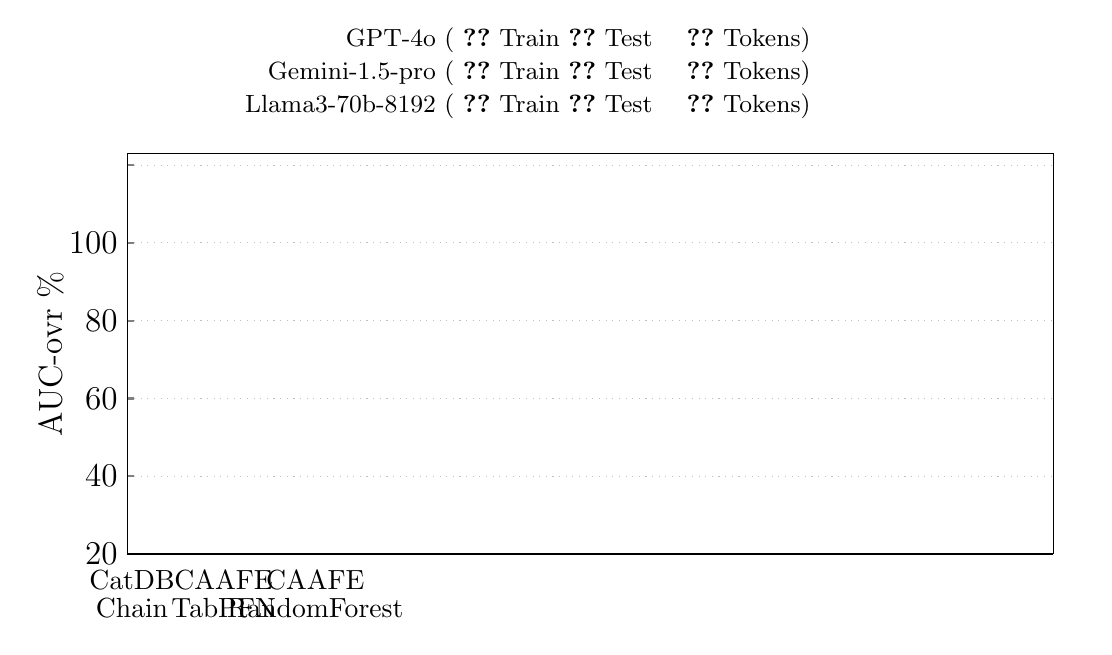
\begin{tikzpicture}[
  every axis/.style={
  height=0.55\columnwidth,
  width=1.1\columnwidth,  
  }]
 \begin{axis}[   
  axis y line*=left,	
  every major tick/.append style={ thick,major tick length=2.5pt, gray},
  axis line style={black},
  ybar,        
  ybar=0pt,
  ymin=0,
  ymax=1,
  log ticks with fixed point,
  y tick label style={/pgf/number format/1000 sep={}},
  x tick label style={/pgf/number format/1000 sep={}},
  scaled y ticks=false,
  enlarge y limits={0.03,upper},
  enlarge x limits=0.005,
  ylabel={AUC-ovr $\%$},
  xlabel={},
  ytick={0,0.2,0.4,0.6,0.8,1.0},
  yticklabels={0, 20, 40, 60, 80, 100},
  xtick style={draw=none},
  xtick pos=left,
  ytick pos=left,
  yticklabel style = {font=\large},
  ylabel style = {font=\large, yshift=-5pt},
  xticklabel style = {font=\normalsize, xshift=0pt, yshift=0pt, rotate=0},
  ymajorgrids,
  grid style=dotted,
  minor grid style={gray!80, dotted},
  nodes near coords,
  every node near coord/.style={font=\fontsize{0.1pt}{0.1}, rotate=0},
  every axis plot/.append style={line width=0.8pt,mark options={scale=1.5,solid}},  
  legend image post style={line width=.5pt},   
  boxplot/draw direction=y,
  boxplot={
      draw position={1 + floor(\plotnumofactualtype/24)+ 1/1*fpumod(\plotnumofactualtype,24)},
      box extend=0.85,
  },
  xtick={3,9,15,22},
  xticklabels={CatDB,\shortstack[c]{CatDB\\Chain},\shortstack[c]{CAAFE\\TabPFN},\shortstack[c]{CAAFE\\RandomForest}},
  legend image code/.code={\draw [#1] (0cm,-0.1cm) rectangle (0.2cm,0.1cm); },  
%}
]  
  \addboxplot{CatDB}{Balance-Scale}{gpt-4o}{}{dblue2}{dblue1};
  \addboxplot{CatDB}{Balance-Scale}{gemini-1.5-pro-latest}{}{dred2}{dred1};
  \addboxplot{CatDB}{Balance-Scale}{llama3-70b-8192}{}{teal2}{teal1};
  

  \addboxplot{CatDBChain}{Balance-Scale}{gpt-4o}{}{dblue2}{dblue1}
  \addboxplot{CatDBChain}{Balance-Scale}{gemini-1.5-pro-latest}{}{dred2}{dred1};
  \addboxplot{CatDBChain}{Balance-Scale}{llama3-70b-8192}{}{teal2}{teal1};
  

  \addboxplot{CAAFE}{Balance-Scale}{gpt-4o}{-TabPFN}{dblue2}{dblue1};
  \addboxplot{CAAFE}{Balance-Scale}{gemini-1.5-pro-latest}{-TabPFN}{dred2}{dred1};
  \addboxplot{CAAFE}{Balance-Scale}{llama3-70b-8192}{-TabPFN}{teal2}{teal1};
  
  \addboxplot{CAAFE}{Balance-Scale}{gpt-4o}{-RandomForest}{dblue2}{dblue1};
  \addboxplot{CAAFE}{Balance-Scale}{gemini-1.5-pro-latest}{-RandomForest}{dred2}{dred1};
  \addboxplot{CAAFE}{Balance-Scale}{llama3-70b-8192}{-RandomForest}{teal2}{teal1};
  
  \coordinate (top1) at (axis cs:6.49,\pgfkeysvalueof{/pgfplots/ymax});
  \coordinate (bot1) at (axis cs:6.49,\pgfkeysvalueof{/pgfplots/ymin});

  \coordinate (top2) at (axis cs:12.49,\pgfkeysvalueof{/pgfplots/ymax});
  \coordinate (bot2) at (axis cs:12.49,\pgfkeysvalueof{/pgfplots/ymin});

  \coordinate (top3) at (axis cs:18.49,\pgfkeysvalueof{/pgfplots/ymax});
  \coordinate (bot3) at (axis cs:18.49,\pgfkeysvalueof{/pgfplots/ymin});

  \draw[black!50, thick] (top1) -- (bot1);
  \draw[black!50, thick] (top2) -- (bot2);
  \draw[black!50, thick] (top3) -- (bot3);

  \draw[gray, densely dotted] (axis cs:2.5,\pgfkeysvalueof{/pgfplots/ymax}) -- (axis cs:2.5,\pgfkeysvalueof{/pgfplots/ymin});
  \draw[gray, densely dotted] (axis cs:4.45,\pgfkeysvalueof{/pgfplots/ymax}) -- (axis cs:4.45,\pgfkeysvalueof{/pgfplots/ymin});

  \draw[gray, densely dotted] (axis cs:8.55,\pgfkeysvalueof{/pgfplots/ymax}) -- (axis cs:8.55,\pgfkeysvalueof{/pgfplots/ymin});
  \draw[gray, densely dotted] (axis cs:10.5,\pgfkeysvalueof{/pgfplots/ymax}) -- (axis cs:10.5,\pgfkeysvalueof{/pgfplots/ymin});

  \draw[gray, densely dotted] (axis cs:14.6,\pgfkeysvalueof{/pgfplots/ymax}) -- (axis cs:14.6,\pgfkeysvalueof{/pgfplots/ymin});
  \draw[gray, densely dotted] (axis cs:16.55,\pgfkeysvalueof{/pgfplots/ymax}) -- (axis cs:16.55,\pgfkeysvalueof{/pgfplots/ymin});

  \draw[gray, densely dotted] (axis cs:20.65,\pgfkeysvalueof{/pgfplots/ymax}) -- (axis cs:20.65,\pgfkeysvalueof{/pgfplots/ymin});
  \draw[gray, densely dotted] (axis cs:22.6,\pgfkeysvalueof{/pgfplots/ymax}) -- (axis cs:22.6,\pgfkeysvalueof{/pgfplots/ymin});

\end{axis}

\begin{axis}[
  axis y line*=right,
  axis x line=none,  
  ybar,  
  ymin=0.5,
  y tick label style={/pgf/number format/1000 sep={}},
  x tick label style={/pgf/number format/1000 sep={}},
  scaled y ticks=false,
  enlarge y limits={1.3,upper},
  enlarge x limits=0.164,
  ylabel={},
  xlabel={},
  ytick={},
  yticklabels={},
  ytick style={draw=none},
  ytick align=outside,
  nodes near coords,
  nodes near coords align={vertical},
  every node near coord/.append style={font=\fontsize{7.5pt}{0.1}, rotate=90, xshift=-11pt, yshift=-6pt},%, rotate=90, xshift=-10pt, yshift=-5pt
  every axis plot/.append style={line width=0.8pt,mark options={scale=1.5,solid}},  
  legend image post style={line width=.5pt},   
  boxplot/draw direction=y,
  bar width=15pt,
  xtick = data,
  symbolic x coords={CatDB,CatDBChain, CAAFETabPFN,CAAFERandomForest},
  legend image code/.code={\draw [#1] (0cm,-0.1cm) rectangle (0.2cm,0.1cm); }, 
  ]   

    \addcost{Balance-Scale}{gpt-4o}{color4!10}{-.5pt};
    \addcost{Balance-Scale}{gemini-1.5-pro-latest}{color4!60}{0.5pt};
    \addcost{Balance-Scale}{llama3-70b-8192}{color4}{1.4pt};
    
\end{axis}

\node [draw=none,inner sep=0, font=\small, anchor=west] (leg1) at (rel axis cs: 0.25,1.20) {\shortstack[r]{
  GPT-4o ( \ref{gpt-4o_CatDB_train} Train \ref{gpt-4o_CatDB_test} Test \ \ \ \ref{gpt-4o} Tokens) \\
  Gemini-1.5-pro ( \ref{gemini-1.5-pro-latest_CatDB_train} Train \ref{gemini-1.5-pro-latest_CatDB_test} Test \ \ \ \ref{gemini-1.5-pro-latest} Tokens) \\
  Llama3-70b-8192 ( \ref{llama3-70b-8192_CatDB_train} Train \ref{llama3-70b-8192_CatDB_test} Test \ \ \ \ref{llama3-70b-8192} Tokens)  
  }};

\end{tikzpicture}
            \caption{Experiment1-Performance-Balance-Scale}
        \end{figure}  
    
  
    \tikzsetnextfilename{Experiment1-Performance-Breast-w} 
        \begin{figure}[!ht]
            \centering
            \pgfmathdeclarefunction{fpumod}{2}{%
        \pgfmathfloatdivide{#1}{#2}%
        \pgfmathfloatint{\pgfmathresult}%
        \pgfmathfloatmultiply{\pgfmathresult}{#2}%
        \pgfmathfloatsubtract{#1}{\pgfmathresult}%
        % replaced `0' by `5' to make it work for this problem
        \pgfmathfloatifapproxequalrel{\pgfmathresult}{#2}{\def\pgfmathresult{5}}{}%
}

\newcommand{\myaddplot}[6]{
  \addplot[xshift=0pt,boxplot,fill=#4, draw=#4, mark options={scale=0.5, fill=#4}, line width=1.5pt] 
  table[y=#2, col sep=comma, x=ID]{#3};
  \label{#5_#6_#1}    
};
    
\newcommand{\addboxplot}[6]{
  \myaddplot{train}{train_auc}{../archive/SIGMOD2025-Results/seperate/#1-#2-#3#4-0-No.csv}{#5}{#3}{#1};
  \myaddplot{test}{test_auc}{../archive/SIGMOD2025-Results/seperate/#1-#2-#3#4-0-No.csv}{#6}{#3}{#1};
};

\newcommand{\myaddplotcost}[4]{ %postaction={pattern=horizontal lines, pattern color=#3}
  \addplot[xshift=#4,fill=#3, draw=black,line width=0.3pt] table[x=config, col sep=comma, y=tokens_count, discard if singlconfig={#1}{#2}]{../archive/SIGMOD2025-Results/CostResults.csv};
  \label{#2}    
};

\newcommand{\addcost}[4]{
  \myaddplotcost{#1}{#2}{#3}{#4};
};


\pgfplotsset{
    discard if singlconfig/.style n args={2}{
        x filter/.code={
            \edef\tempa{\thisrow{dataset_name_orig}}
            \edef\tempb{#1}
            \ifx\tempa\tempb
              \edef\tempc{\thisrow{llm_model}}
                \edef\tempd{#2}
                  \ifx\tempc\tempd                  
                  \else
                  \def\pgfmathresult{inf}
                  \fi
            \else
            \def\pgfmathresult{inf}
            \fi			
        }
    },
};

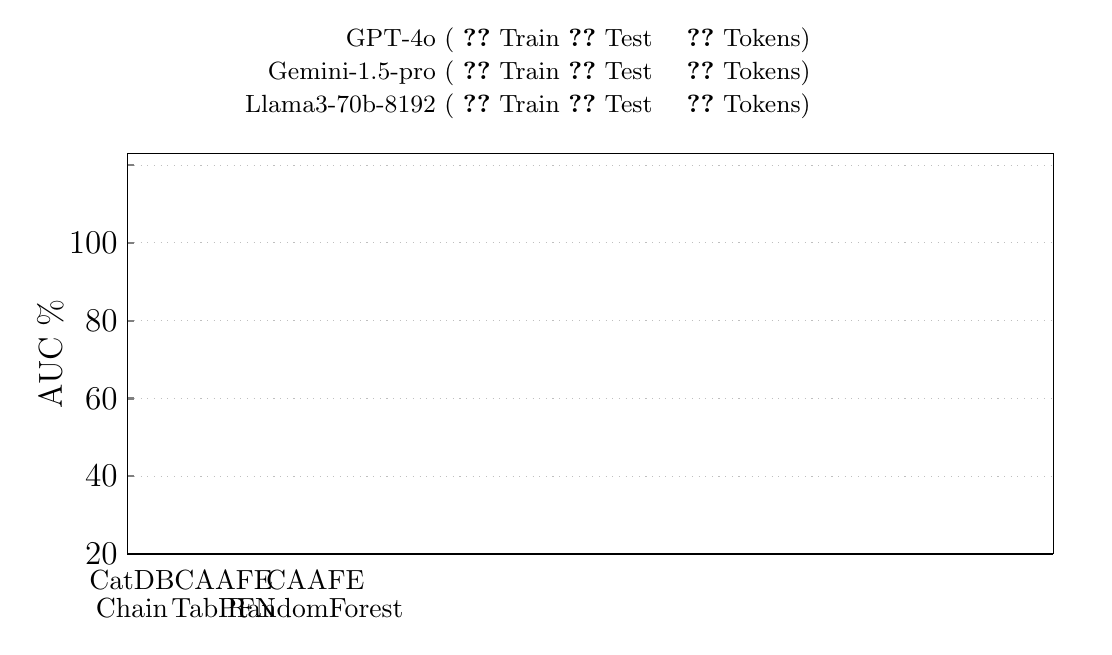
\begin{tikzpicture}[
  every axis/.style={
  height=0.55\columnwidth,
  width=1.1\columnwidth,  
  }]
 \begin{axis}[   
  axis y line*=left,	
  every major tick/.append style={ thick,major tick length=2.5pt, gray},
  axis line style={black},
  ybar,        
  ybar=0pt,
  ymin=0,
  ymax=1,
  log ticks with fixed point,
  y tick label style={/pgf/number format/1000 sep={}},
  x tick label style={/pgf/number format/1000 sep={}},
  scaled y ticks=false,
  enlarge y limits={0.03,upper},
  enlarge x limits=0.005,
  ylabel={AUC $\%$},
  xlabel={},
  ytick={0,0.2,0.4,0.6,0.8,1.0},
  yticklabels={0, 20, 40, 60, 80, 100},
  xtick style={draw=none},
  xtick pos=left,
  ytick pos=left,
  yticklabel style = {font=\large},
  ylabel style = {font=\large, yshift=-5pt},
  xticklabel style = {font=\normalsize, xshift=0pt, yshift=0pt, rotate=0},
  ymajorgrids,
  grid style=dotted,
  minor grid style={gray!80, dotted},
  nodes near coords,
  every node near coord/.style={font=\fontsize{0.1pt}{0.1}, rotate=0},
  every axis plot/.append style={line width=0.8pt,mark options={scale=1.5,solid}},  
  legend image post style={line width=.5pt},   
  boxplot/draw direction=y,
  boxplot={
      draw position={1 + floor(\plotnumofactualtype/24)+ 1/1*fpumod(\plotnumofactualtype,24)},
      box extend=0.85,
  },
  xtick={3,9,15,22},
  xticklabels={CatDB,\shortstack[c]{CatDB\\Chain},\shortstack[c]{CAAFE\\TabPFN},\shortstack[c]{CAAFE\\RandomForest}},
  legend image code/.code={\draw [#1] (0cm,-0.1cm) rectangle (0.2cm,0.1cm); },  
%}
]  
  \addboxplot{CatDB}{Breast-w}{gpt-4o}{}{dblue2}{dblue1};
  \addboxplot{CatDB}{Breast-w}{gemini-1.5-pro-latest}{}{dred2}{dred1};
  \addboxplot{CatDB}{Breast-w}{llama3-70b-8192}{}{teal2}{teal1};
  

  \addboxplot{CatDBChain}{Breast-w}{gpt-4o}{}{dblue2}{dblue1}
  \addboxplot{CatDBChain}{Breast-w}{gemini-1.5-pro-latest}{}{dred2}{dred1};
  \addboxplot{CatDBChain}{Breast-w}{llama3-70b-8192}{}{teal2}{teal1};
  

  \addboxplot{CAAFE}{Breast-w}{gpt-4o}{-TabPFN}{dblue2}{dblue1};
  \addboxplot{CAAFE}{Breast-w}{gemini-1.5-pro-latest}{-TabPFN}{dred2}{dred1};
  \addboxplot{CAAFE}{Balance-Scale}{llama3-70b-8192}{-TabPFN}{teal2}{teal1};
  
  \addboxplot{CAAFE}{Breast-w}{gpt-4o}{-RandomForest}{dblue2}{dblue1};
  \addboxplot{CAAFE}{Breast-w}{gemini-1.5-pro-latest}{-RandomForest}{dred2}{dred1};
  \addboxplot{CAAFE}{Breast-w}{llama3-70b-8192}{-RandomForest}{teal2}{teal1};
  
  \coordinate (top1) at (axis cs:6.49,\pgfkeysvalueof{/pgfplots/ymax});
  \coordinate (bot1) at (axis cs:6.49,\pgfkeysvalueof{/pgfplots/ymin});

  \coordinate (top2) at (axis cs:12.49,\pgfkeysvalueof{/pgfplots/ymax});
  \coordinate (bot2) at (axis cs:12.49,\pgfkeysvalueof{/pgfplots/ymin});

  \coordinate (top3) at (axis cs:18.49,\pgfkeysvalueof{/pgfplots/ymax});
  \coordinate (bot3) at (axis cs:18.49,\pgfkeysvalueof{/pgfplots/ymin});

  \draw[black!50, thick] (top1) -- (bot1);
  \draw[black!50, thick] (top2) -- (bot2);
  \draw[black!50, thick] (top3) -- (bot3);

  \draw[gray, densely dotted] (axis cs:2.5,\pgfkeysvalueof{/pgfplots/ymax}) -- (axis cs:2.5,\pgfkeysvalueof{/pgfplots/ymin});
  \draw[gray, densely dotted] (axis cs:4.45,\pgfkeysvalueof{/pgfplots/ymax}) -- (axis cs:4.45,\pgfkeysvalueof{/pgfplots/ymin});

  \draw[gray, densely dotted] (axis cs:8.55,\pgfkeysvalueof{/pgfplots/ymax}) -- (axis cs:8.55,\pgfkeysvalueof{/pgfplots/ymin});
  \draw[gray, densely dotted] (axis cs:10.5,\pgfkeysvalueof{/pgfplots/ymax}) -- (axis cs:10.5,\pgfkeysvalueof{/pgfplots/ymin});

  \draw[gray, densely dotted] (axis cs:14.6,\pgfkeysvalueof{/pgfplots/ymax}) -- (axis cs:14.6,\pgfkeysvalueof{/pgfplots/ymin});
  \draw[gray, densely dotted] (axis cs:16.55,\pgfkeysvalueof{/pgfplots/ymax}) -- (axis cs:16.55,\pgfkeysvalueof{/pgfplots/ymin});

  \draw[gray, densely dotted] (axis cs:20.65,\pgfkeysvalueof{/pgfplots/ymax}) -- (axis cs:20.65,\pgfkeysvalueof{/pgfplots/ymin});
  \draw[gray, densely dotted] (axis cs:22.6,\pgfkeysvalueof{/pgfplots/ymax}) -- (axis cs:22.6,\pgfkeysvalueof{/pgfplots/ymin});

\end{axis}

\begin{axis}[
  axis y line*=right,
  axis x line=none,  
  ybar,  
  ymin=0.5,
  y tick label style={/pgf/number format/1000 sep={}},
  x tick label style={/pgf/number format/1000 sep={}},
  scaled y ticks=false,
  enlarge y limits={1.3,upper},
  enlarge x limits=0.164,
  ylabel={},
  xlabel={},
  ytick={},
  yticklabels={},
  ytick style={draw=none},
  ytick align=outside,
  nodes near coords,
  nodes near coords align={vertical},
  every node near coord/.append style={font=\fontsize{7.5pt}{0.1}, rotate=90, xshift=-11pt, yshift=-6pt},%, rotate=90, xshift=-10pt, yshift=-5pt
  every axis plot/.append style={line width=0.8pt,mark options={scale=1.5,solid}},  
  legend image post style={line width=.5pt},   
  boxplot/draw direction=y,
  bar width=15pt,
  xtick = data,
  symbolic x coords={CatDB,CatDBChain, CAAFETabPFN,CAAFERandomForest},
  legend image code/.code={\draw [#1] (0cm,-0.1cm) rectangle (0.2cm,0.1cm); }, 
  ]   

    \addcost{Breast-w}{gpt-4o}{color4!10}{-.5pt};
    \addcost{Breast-w}{gemini-1.5-pro-latest}{color4!60}{0.5pt};
    \addcost{Breast-w}{llama3-70b-8192}{color4}{1.4pt};
    
\end{axis}

\node [draw=none,inner sep=0, font=\small, anchor=west] (leg1) at (rel axis cs: 0.25,1.20) {\shortstack[r]{
  GPT-4o ( \ref{gpt-4o_CatDB_train} Train \ref{gpt-4o_CatDB_test} Test \ \ \ \ref{gpt-4o} Tokens) \\
  Gemini-1.5-pro ( \ref{gemini-1.5-pro-latest_CatDB_train} Train \ref{gemini-1.5-pro-latest_CatDB_test} Test \ \ \ \ref{gemini-1.5-pro-latest} Tokens) \\
  Llama3-70b-8192 ( \ref{llama3-70b-8192_CatDB_train} Train \ref{llama3-70b-8192_CatDB_test} Test \ \ \ \ref{llama3-70b-8192} Tokens)  
  }};

\end{tikzpicture}
            \caption{Experiment1-Performance-Breast-w}
        \end{figure}  
    
  
    \tikzsetnextfilename{Experiment1-Performance-CMC} 
        \begin{figure}[!ht]
            \centering
            \pgfmathdeclarefunction{fpumod}{2}{%
        \pgfmathfloatdivide{#1}{#2}%
        \pgfmathfloatint{\pgfmathresult}%
        \pgfmathfloatmultiply{\pgfmathresult}{#2}%
        \pgfmathfloatsubtract{#1}{\pgfmathresult}%
        % replaced `0' by `5' to make it work for this problem
        \pgfmathfloatifapproxequalrel{\pgfmathresult}{#2}{\def\pgfmathresult{5}}{}%
}

\newcommand{\myaddplot}[6]{
  \addplot[xshift=0pt,boxplot,fill=#4, draw=#4, mark options={scale=0.5, fill=#4}, line width=1.5pt] 
  table[y=#2, col sep=comma, x=ID]{#3};
  \label{#5_#6_#1}    
};
    
\newcommand{\addboxplot}[6]{
  \myaddplot{train}{train_auc_ovr}{../archive/SIGMOD2025-Results/seperate/#1-#2-#3#4-0-No.csv}{#5}{#3}{#1};
  \myaddplot{test}{test_auc_ovr}{../archive/SIGMOD2025-Results/seperate/#1-#2-#3#4-0-No.csv}{#6}{#3}{#1};
};

\newcommand{\myaddplotcost}[4]{ %postaction={pattern=horizontal lines, pattern color=#3}
  \addplot[xshift=#4,fill=#3, draw=black,line width=0.3pt] table[x=config, col sep=comma, y=tokens_count, discard if singlconfig={#1}{#2}]{../archive/SIGMOD2025-Results/CostResults.csv};
  \label{#2}    
};

\newcommand{\addcost}[4]{
  \myaddplotcost{#1}{#2}{#3}{#4};
};


\pgfplotsset{
    discard if singlconfig/.style n args={2}{
        x filter/.code={
            \edef\tempa{\thisrow{dataset_name_orig}}
            \edef\tempb{#1}
            \ifx\tempa\tempb
              \edef\tempc{\thisrow{llm_model}}
                \edef\tempd{#2}
                  \ifx\tempc\tempd                  
                  \else
                  \def\pgfmathresult{inf}
                  \fi
            \else
            \def\pgfmathresult{inf}
            \fi			
        }
    },
};

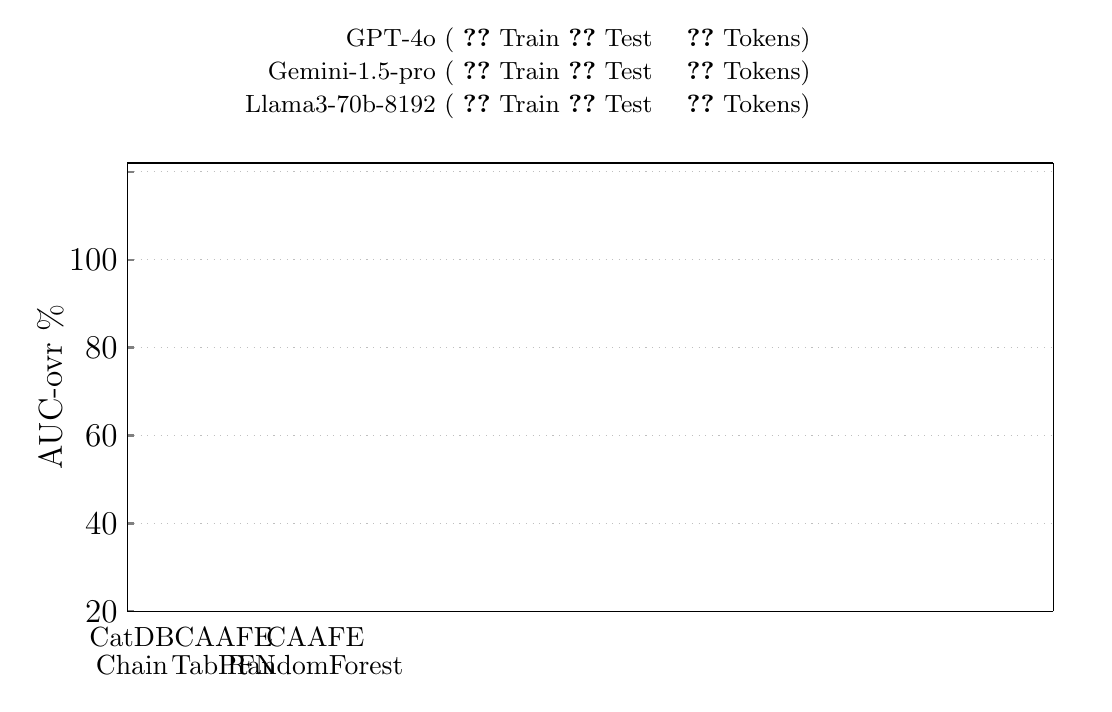
\begin{tikzpicture}[
  every axis/.style={
  height=0.6\columnwidth,
  width=1.1\columnwidth,  
  }]
 \begin{axis}[   
  axis y line*=left,	
  every major tick/.append style={ thick,major tick length=2.5pt, gray},
  axis line style={black},
  ybar,        
  ybar=0pt,
  ymin=0,
  ymax=1,
  log ticks with fixed point,
  y tick label style={/pgf/number format/1000 sep={}},
  x tick label style={/pgf/number format/1000 sep={}},
  scaled y ticks=false,
  enlarge y limits={0.02,upper},
  enlarge x limits=0.005,
  ylabel={AUC-ovr $\%$},
  xlabel={},
  ytick={0,0.2,0.4,0.6,0.8,1.0},
  yticklabels={0, 20, 40, 60, 80, 100},
  xtick style={draw=none},
  xtick pos=left,
  ytick pos=left,
  yticklabel style = {font=\large},
  ylabel style = {font=\large, yshift=-5pt},
  xticklabel style = {font=\normalsize, xshift=0pt, yshift=0pt, rotate=0},
  ymajorgrids,
  grid style=dotted,
  minor grid style={gray!80, dotted},
  nodes near coords,
  every node near coord/.style={font=\fontsize{0.1pt}{0.1}, rotate=0},
  every axis plot/.append style={line width=0.8pt,mark options={scale=1.5,solid}},  
  legend image post style={line width=.5pt},   
  boxplot/draw direction=y,
  boxplot={
      draw position={1 + floor(\plotnumofactualtype/24)+ 1/1*fpumod(\plotnumofactualtype,24)},
      box extend=0.85,
  },
  xtick={3,9,15,22},
  xticklabels={CatDB,\shortstack[c]{CatDB\\Chain},\shortstack[c]{CAAFE\\TabPFN},\shortstack[c]{CAAFE\\RandomForest}},
  legend image code/.code={\draw [#1] (0cm,-0.1cm) rectangle (0.2cm,0.1cm); },  
%}
]  
  \addboxplot{CatDB}{CMC}{gpt-4o}{}{dblue2}{dblue1};
  \addboxplot{CatDB}{CMC}{gemini-1.5-pro-latest}{}{dred2}{dred1};
  \addboxplot{CatDB}{CMC}{llama3-70b-8192}{}{teal2}{teal1};
  

  \addboxplot{CatDBChain}{CMC}{gpt-4o}{}{dblue2}{dblue1}
  \addboxplot{CatDBChain}{CMC}{gemini-1.5-pro-latest}{}{dred2}{dred1};
  \addboxplot{CatDBChain}{CMC}{llama3-70b-8192}{}{teal2}{teal1};
  

  \addboxplot{CAAFE}{CMC}{gpt-4o}{-TabPFN}{dblue2}{dblue1};
  \addboxplot{CAAFE}{CMC}{gemini-1.5-pro-latest}{-TabPFN}{dred2}{dred1};
  \addboxplot{CAAFE}{Balance-Scale}{llama3-70b-8192}{-TabPFN}{teal2}{teal1};
  
  \addboxplot{CAAFE}{CMC}{gpt-4o}{-RandomForest}{dblue2}{dblue1};
  \addboxplot{CAAFE}{CMC}{gemini-1.5-pro-latest}{-RandomForest}{dred2}{dred1};
  \addboxplot{CAAFE}{CMC}{llama3-70b-8192}{-RandomForest}{teal2}{teal1};
  
  \coordinate (top1) at (axis cs:6.49,\pgfkeysvalueof{/pgfplots/ymax});
  \coordinate (bot1) at (axis cs:6.49,\pgfkeysvalueof{/pgfplots/ymin});

  \coordinate (top2) at (axis cs:12.49,\pgfkeysvalueof{/pgfplots/ymax});
  \coordinate (bot2) at (axis cs:12.49,\pgfkeysvalueof{/pgfplots/ymin});

  \coordinate (top3) at (axis cs:18.49,\pgfkeysvalueof{/pgfplots/ymax});
  \coordinate (bot3) at (axis cs:18.49,\pgfkeysvalueof{/pgfplots/ymin});

  \draw[black!50, thick] (top1) -- (bot1);
  \draw[black!50, thick] (top2) -- (bot2);
  \draw[black!50, thick] (top3) -- (bot3);

  \draw[gray, densely dotted] (axis cs:2.5,\pgfkeysvalueof{/pgfplots/ymax}) -- (axis cs:2.5,\pgfkeysvalueof{/pgfplots/ymin});
  \draw[gray, densely dotted] (axis cs:4.45,\pgfkeysvalueof{/pgfplots/ymax}) -- (axis cs:4.45,\pgfkeysvalueof{/pgfplots/ymin});

  \draw[gray, densely dotted] (axis cs:8.55,\pgfkeysvalueof{/pgfplots/ymax}) -- (axis cs:8.55,\pgfkeysvalueof{/pgfplots/ymin});
  \draw[gray, densely dotted] (axis cs:10.5,\pgfkeysvalueof{/pgfplots/ymax}) -- (axis cs:10.5,\pgfkeysvalueof{/pgfplots/ymin});

  \draw[gray, densely dotted] (axis cs:14.6,\pgfkeysvalueof{/pgfplots/ymax}) -- (axis cs:14.6,\pgfkeysvalueof{/pgfplots/ymin});
  \draw[gray, densely dotted] (axis cs:16.55,\pgfkeysvalueof{/pgfplots/ymax}) -- (axis cs:16.55,\pgfkeysvalueof{/pgfplots/ymin});

  \draw[gray, densely dotted] (axis cs:20.65,\pgfkeysvalueof{/pgfplots/ymax}) -- (axis cs:20.65,\pgfkeysvalueof{/pgfplots/ymin});
  \draw[gray, densely dotted] (axis cs:22.6,\pgfkeysvalueof{/pgfplots/ymax}) -- (axis cs:22.6,\pgfkeysvalueof{/pgfplots/ymin});

\end{axis}

\begin{axis}[
  axis y line*=right,
  axis x line=none,  
  ybar,  
  ymin=0.5,
  y tick label style={/pgf/number format/1000 sep={}},
  x tick label style={/pgf/number format/1000 sep={}},
  scaled y ticks=false,
  enlarge y limits={0.97,upper},
  enlarge x limits=0.164,
  ylabel={},
  xlabel={},
  ytick={},
  yticklabels={},
  ytick style={draw=none},
  ytick align=outside,
  nodes near coords,
  nodes near coords align={vertical},
  every node near coord/.append style={font=\fontsize{7.5pt}{0.1}, rotate=90, xshift=-11pt, yshift=-6pt},%, rotate=90, xshift=-10pt, yshift=-5pt
  every axis plot/.append style={line width=0.8pt,mark options={scale=1.5,solid}},  
  legend image post style={line width=.5pt},   
  boxplot/draw direction=y,
  bar width=15pt,
  xtick = data,
  symbolic x coords={CatDB,CatDBChain, CAAFETabPFN,CAAFERandomForest},
  legend image code/.code={\draw [#1] (0cm,-0.1cm) rectangle (0.2cm,0.1cm); }, 
  ]   

    \addcost{CMC}{gpt-4o}{color4!10}{-.5pt};
    \addcost{CMC}{gemini-1.5-pro-latest}{color4!60}{0.5pt};
    \addcost{CMC}{llama3-70b-8192}{color4}{1.4pt};
    
\end{axis}

\node [draw=none,inner sep=0, font=\small, anchor=west] (leg1) at (rel axis cs: 0.25,1.20) {\shortstack[r]{
  GPT-4o ( \ref{gpt-4o_CatDB_train} Train \ref{gpt-4o_CatDB_test} Test \ \ \ \ref{gpt-4o} Tokens) \\
  Gemini-1.5-pro ( \ref{gemini-1.5-pro-latest_CatDB_train} Train \ref{gemini-1.5-pro-latest_CatDB_test} Test \ \ \ \ref{gemini-1.5-pro-latest} Tokens) \\
  Llama3-70b-8192 ( \ref{llama3-70b-8192_CatDB_train} Train \ref{llama3-70b-8192_CatDB_test} Test \ \ \ \ref{llama3-70b-8192} Tokens)  
  }};

\end{tikzpicture}
            \caption{Experiment1-Performance-CMC}
        \end{figure}  
    
  
    \tikzsetnextfilename{Experiment1-Performance-Credit-g} 
        \begin{figure}[!ht]
            \centering
            \pgfmathdeclarefunction{fpumod}{2}{%
        \pgfmathfloatdivide{#1}{#2}%
        \pgfmathfloatint{\pgfmathresult}%
        \pgfmathfloatmultiply{\pgfmathresult}{#2}%
        \pgfmathfloatsubtract{#1}{\pgfmathresult}%
        % replaced `0' by `5' to make it work for this problem
        \pgfmathfloatifapproxequalrel{\pgfmathresult}{#2}{\def\pgfmathresult{5}}{}%
}

\newcommand{\myaddplot}[6]{
  \addplot[xshift=0pt,boxplot,fill=#4, draw=#4, mark options={scale=0.5, fill=#4}, line width=1.5pt] 
  table[y=#2, col sep=comma, x=ID]{#3};
  \label{#5_#6_#1}    
};
    
\newcommand{\addboxplot}[6]{
  \myaddplot{train}{train_auc}{../archive/SIGMOD2025-Results/seperate/#1-#2-#3#4-No.csv}{#5}{#3}{#1};
  \myaddplot{test}{test_auc}{../archive/SIGMOD2025-Results/seperate/#1-#2-#3#4-No.csv}{#6}{#3}{#1};
};

\newcommand{\myaddplotcost}[4]{ %postaction={pattern=horizontal lines, pattern color=#3}
  \addplot[xshift=#4,fill=#3, draw=black,line width=0.3pt] table[x=config, col sep=comma, y=tokens_count, discard if singlconfig={#1}{#2}]{../archive/SIGMOD2025-Results/CostResults.csv};
  \label{#2}    
};

\newcommand{\addcost}[4]{
  \myaddplotcost{#1}{#2}{#3}{#4};
};


\pgfplotsset{
    discard if singlconfig/.style n args={2}{
        x filter/.code={
            \edef\tempa{\thisrow{dataset_name_orig}}
            \edef\tempb{#1}
            \ifx\tempa\tempb
              \edef\tempc{\thisrow{llm_model}}
                \edef\tempd{#2}
                  \ifx\tempc\tempd                  
                  \else
                  \def\pgfmathresult{inf}
                  \fi
            \else
            \def\pgfmathresult{inf}
            \fi			
        }
    },
};

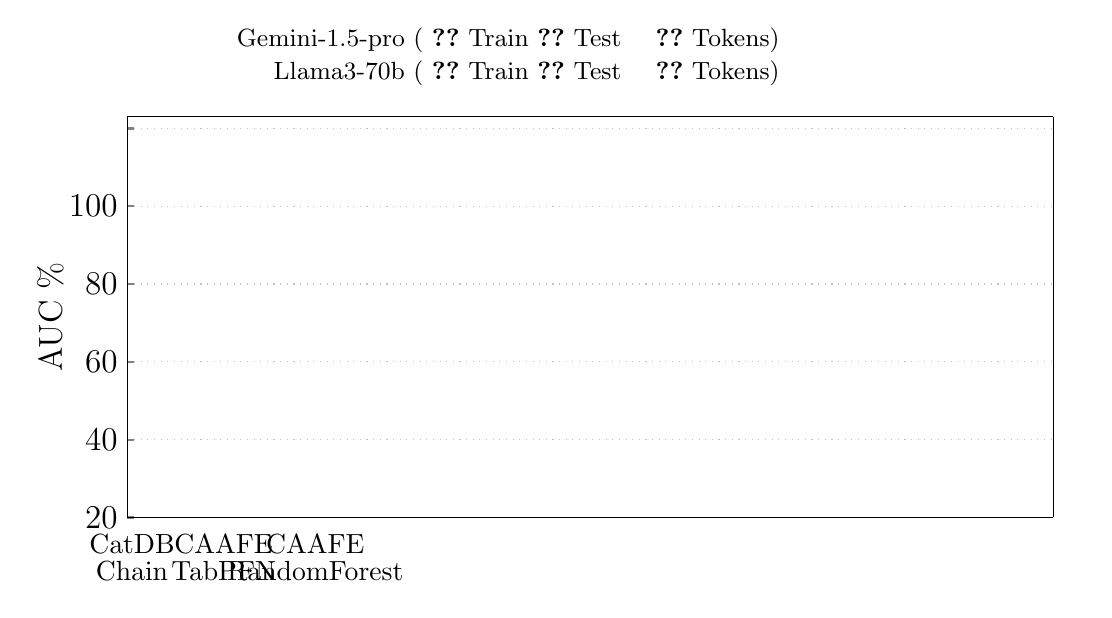
\begin{tikzpicture}[
  every axis/.style={
  height=0.55\columnwidth,
  width=1.1\columnwidth,  
  }]
 \begin{axis}[   
  axis y line*=left,	
  every major tick/.append style={ thick,major tick length=2.5pt, gray},
  axis line style={black},
  ybar,        
  ybar=0pt,
  ymin=0,
  ymax=1,
  log ticks with fixed point,
  y tick label style={/pgf/number format/1000 sep={}},
  x tick label style={/pgf/number format/1000 sep={}},
  scaled y ticks=false,
  enlarge y limits={0.03,upper},
  enlarge x limits=0.005,
  ylabel={AUC $\%$},
  xlabel={},
  ytick={0,0.2,0.4,0.6,0.8,1.0},
  yticklabels={0, 20, 40, 60, 80, 100},
  xtick style={draw=none},
  xtick pos=left,
  ytick pos=left,
  yticklabel style = {font=\large},
  ylabel style = {font=\large, yshift=-5pt},
  xticklabel style = {font=\normalsize, xshift=0pt, yshift=0pt, rotate=0},
  ymajorgrids,
  grid style=dotted,
  minor grid style={gray!80, dotted},
  nodes near coords,
  every node near coord/.style={font=\fontsize{0.1pt}{0.1}, rotate=0},
  every axis plot/.append style={line width=0.8pt,mark options={scale=1.5,solid}},  
  legend image post style={line width=.5pt},   
  boxplot/draw direction=y,
  boxplot={
      draw position={1 + floor(\plotnumofactualtype/24)+ 1/1*fpumod(\plotnumofactualtype,24)},
      box extend=0.85,
  },
  xtick={3,9,15,22},
  xticklabels={CatDB,\shortstack[c]{CatDB\\Chain},\shortstack[c]{CAAFE\\TabPFN},\shortstack[c]{CAAFE\\RandomForest}},
  legend image code/.code={\draw [#1] (0cm,-0.1cm) rectangle (0.2cm,0.1cm); },  
%}
]  
  \addboxplot{CatDB}{Credit-g-rnc}{gemini-1.5-pro-latest}{}{white}{white}; %{color4!60}{color4}
  \addboxplot{CatDB}{Credit-g-rnc}{gemini-1.5-pro-latest}{}{tug!50}{tug};
  \addboxplot{CatDB}{Credit-g-rnc}{llama3-70b-8192}{}{tugb}{tugb!150};
  

  \addboxplot{CatDBChain}{Credit-g-rnc}{gemini-1.5-pro-latest}{}{white}{white};
  \addboxplot{CatDBChain}{Credit-g-rnc}{gemini-1.5-pro-latest}{}{tug!50}{tug};
  \addboxplot{CatDBChain}{Credit-g-rnc}{llama3-70b-8192}{}{tugb}{tugb!150};
  

  \addboxplot{CAAFE}{Credit-g-rnc}{gemini-1.5-pro-latest}{-TabPFN}{white}{white};
  \addboxplot{CAAFE}{Credit-g-rnc}{gemini-1.5-pro-latest}{-TabPFN}{tug!50}{tug};
  \addboxplot{CAAFE}{Credit-g-rnc}{gemini-1.5-pro-latest}{-TabPFN}{white}{white};
  
  \addboxplot{CAAFE}{Credit-g-rnc}{gemini-1.5-pro-latest}{-RandomForest}{white}{white};
  \addboxplot{CAAFE}{Credit-g-rnc}{gemini-1.5-pro-latest}{-RandomForest}{tug!50}{tug};
  \addboxplot{CAAFE}{Credit-g-rnc}{gemini-1.5-pro-latest}{-RandomForest}{white}{white};
  

  \draw[black!50, thick] (59,0) -- (59,103);
  \draw[black!50, thick] (119,0) -- (119,103);
  \draw[black!50, thick] (179,0) -- (179,103);

\end{axis}

\begin{axis}[
  axis y line*=right,
  axis x line=none,  
  ybar,  
  ymin=0.5,
  y tick label style={/pgf/number format/1000 sep={}},
  x tick label style={/pgf/number format/1000 sep={}},
  scaled y ticks=false,
  enlarge y limits={1.3,upper},
  enlarge x limits=0.18,
  ylabel={},
  xlabel={},
  ytick={},
  yticklabels={},
  ytick style={draw=none},
  ytick align=outside,
  nodes near coords,
  nodes near coords align={vertical},
  every node near coord/.append style={font=\fontsize{7.5pt}{0.1}, rotate=90, xshift=-11pt, yshift=-6pt},%, rotate=90, xshift=-10pt, yshift=-5pt
  every axis plot/.append style={line width=0.8pt,mark options={scale=1.5,solid}},  
  legend image post style={line width=.5pt},   
  boxplot/draw direction=y,
  bar width=13pt,
  xtick = data,
  symbolic x coords={CatDB,CatDBChain, CAAFETabPFN,CAAFERandomForest},
  legend image code/.code={\draw [#1] (0cm,-0.1cm) rectangle (0.2cm,0.1cm); }, 
  ]   

    %\addcost{Credit-g-rnc}{gemini-1.5-pro-latest}{color8!10}{0pt};
    \addcost{Credit-g-rnc}{gemini-1.5-pro-latest}{color8!40}{0pt};
    \addcost{Credit-g-rnc}{llama3-70b-8192}{color8!70!}{0pt};
    
\end{axis}

\node [draw=none,inner sep=0, font=\small, anchor=west] (leg1) at (rel axis cs: 0.25,1.15) {\shortstack[r]{
  Gemini-1.5-pro ( \ref{gemini-1.5-pro-latest_CatDB_train} Train \ref{gemini-1.5-pro-latest_CatDB_test} Test \ \ \ \ref{gemini-1.5-pro-latest} Tokens) \\
  Llama3-70b ( \ref{llama3-70b-8192_CatDB_train} Train \ref{llama3-70b-8192_CatDB_test} Test \ \ \ \ref{llama3-70b-8192} Tokens)}};

\end{tikzpicture}
            \caption{Experiment1-Performance-Credit-g}
        \end{figure}  
    
  
    \tikzsetnextfilename{Experiment1-Performance-Diabetes} 
        \begin{figure}[!ht]
            \centering
            \pgfmathdeclarefunction{fpumod}{2}{%
        \pgfmathfloatdivide{#1}{#2}%
        \pgfmathfloatint{\pgfmathresult}%
        \pgfmathfloatmultiply{\pgfmathresult}{#2}%
        \pgfmathfloatsubtract{#1}{\pgfmathresult}%
        % replaced `0' by `5' to make it work for this problem
        \pgfmathfloatifapproxequalrel{\pgfmathresult}{#2}{\def\pgfmathresult{5}}{}%
}

\newcommand{\myaddplot}[6]{
  \addplot[xshift=0pt,boxplot,fill=#4, draw=#4, mark options={scale=0.5, fill=#4}, line width=1.5pt] 
  table[y=#2, col sep=comma, x=ID]{#3};
  \label{#5_#6_#1}    
};
    
\newcommand{\addboxplot}[6]{
  \myaddplot{train}{train_auc}{../archive/SIGMOD2025-Results/seperate/#1-#2-#3#4-No.csv}{#5}{#3}{#1};
  \myaddplot{test}{test_auc}{../archive/SIGMOD2025-Results/seperate/#1-#2-#3#4-No.csv}{#6}{#3}{#1};
};

\newcommand{\myaddplotcost}[4]{ %postaction={pattern=horizontal lines, pattern color=#3}
  \addplot[xshift=#4,fill=#3, draw=black,line width=0.3pt] table[x=config, col sep=comma, y=tokens_count, discard if singlconfig={#1}{#2}]{../archive/SIGMOD2025-Results/CostResults.csv};
  \label{#2}    
};

\newcommand{\addcost}[4]{
  \myaddplotcost{#1}{#2}{#3}{#4};
};


\pgfplotsset{
    discard if singlconfig/.style n args={2}{
        x filter/.code={
            \edef\tempa{\thisrow{dataset_name_orig}}
            \edef\tempb{#1}
            \ifx\tempa\tempb
              \edef\tempc{\thisrow{llm_model}}
                \edef\tempd{#2}
                  \ifx\tempc\tempd                  
                  \else
                  \def\pgfmathresult{inf}
                  \fi
            \else
            \def\pgfmathresult{inf}
            \fi			
        }
    },
};

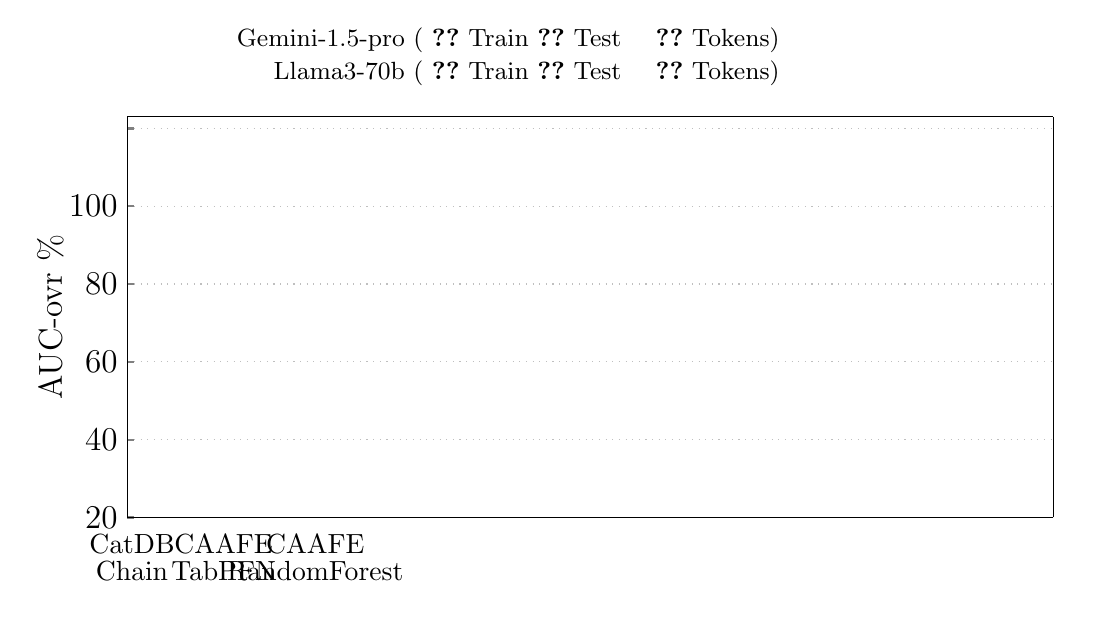
\begin{tikzpicture}[
  every axis/.style={
  height=0.55\columnwidth,
  width=1.1\columnwidth,  
  }]
 \begin{axis}[   
  axis y line*=left,	
  every major tick/.append style={ thick,major tick length=2.5pt, gray},
  axis line style={black},
  ybar,        
  ybar=0pt,
  ymin=0,
  ymax=1,
  log ticks with fixed point,
  y tick label style={/pgf/number format/1000 sep={}},
  x tick label style={/pgf/number format/1000 sep={}},
  scaled y ticks=false,
  enlarge y limits={0.03,upper},
  enlarge x limits=0.005,
  ylabel={AUC-ovr $\%$},
  xlabel={},
  ytick={0,0.2,0.4,0.6,0.8,1.0},
  yticklabels={0, 20, 40, 60, 80, 100},
  xtick style={draw=none},
  xtick pos=left,
  ytick pos=left,
  yticklabel style = {font=\large},
  ylabel style = {font=\large, yshift=-5pt},
  xticklabel style = {font=\normalsize, xshift=0pt, yshift=0pt, rotate=0},
  ymajorgrids,
  grid style=dotted,
  minor grid style={gray!80, dotted},
  nodes near coords,
  every node near coord/.style={font=\fontsize{0.1pt}{0.1}, rotate=0},
  every axis plot/.append style={line width=0.8pt,mark options={scale=1.5,solid}},  
  legend image post style={line width=.5pt},   
  boxplot/draw direction=y,
  boxplot={
      draw position={1 + floor(\plotnumofactualtype/24)+ 1/1*fpumod(\plotnumofactualtype,24)},
      box extend=0.85,
  },
  xtick={3,9,15,22},
  xticklabels={CatDB,\shortstack[c]{CatDB\\Chain},\shortstack[c]{CAAFE\\TabPFN},\shortstack[c]{CAAFE\\RandomForest}},
  legend image code/.code={\draw [#1] (0cm,-0.1cm) rectangle (0.2cm,0.1cm); },  
%}
]  
  \addboxplot{CatDB}{Diabetes-rnc}{gemini-1.5-pro-latest}{}{white}{white}; %{color4!60}{color4}
  \addboxplot{CatDB}{Diabetes-rnc}{gemini-1.5-pro-latest}{}{tug!50}{tug};
  \addboxplot{CatDB}{Diabetes-rnc}{llama3-70b-8192}{}{tugb}{tugb!150};
  

  \addboxplot{CatDBChain}{Diabetes-rnc}{gemini-1.5-pro-latest}{}{white}{white};
  \addboxplot{CatDBChain}{Diabetes-rnc}{gemini-1.5-pro-latest}{}{tug!50}{tug};
  \addboxplot{CatDBChain}{Diabetes-rnc}{llama3-70b-8192}{}{tugb}{tugb!150};
  

  \addboxplot{CAAFE}{Diabetes-rnc}{gemini-1.5-pro-latest}{-TabPFN}{white}{white};
  \addboxplot{CAAFE}{Diabetes-rnc}{gemini-1.5-pro-latest}{-TabPFN}{tug!50}{tug};
  \addboxplot{CAAFE}{Diabetes-rnc}{gemini-1.5-pro-latest}{-TabPFN}{white}{white};
  
  \addboxplot{CAAFE}{Diabetes-rnc}{gemini-1.5-pro-latest}{-RandomForest}{white}{white};
  \addboxplot{CAAFE}{Diabetes-rnc}{gemini-1.5-pro-latest}{-RandomForest}{tug!50}{tug};
  \addboxplot{CAAFE}{Diabetes-rnc}{gemini-1.5-pro-latest}{-RandomForest}{white}{white};
  

  \draw[black!50, thick] (59,0) -- (59,103);
  \draw[black!50, thick] (119,0) -- (119,103);
  \draw[black!50, thick] (179,0) -- (179,103);

\end{axis}

\begin{axis}[
  axis y line*=right,
  axis x line=none,  
  ybar,  
  ymin=0.5,
  y tick label style={/pgf/number format/1000 sep={}},
  x tick label style={/pgf/number format/1000 sep={}},
  scaled y ticks=false,
  enlarge y limits={1.3,upper},
  enlarge x limits=0.18,
  ylabel={},
  xlabel={},
  ytick={},
  yticklabels={},
  ytick style={draw=none},
  ytick align=outside,
  nodes near coords,
  nodes near coords align={vertical},
  every node near coord/.append style={font=\fontsize{7.5pt}{0.1}, rotate=90, xshift=-11pt, yshift=-6pt},%, rotate=90, xshift=-10pt, yshift=-5pt
  every axis plot/.append style={line width=0.8pt,mark options={scale=1.5,solid}},  
  legend image post style={line width=.5pt},   
  boxplot/draw direction=y,
  bar width=13pt,
  xtick = data,
  symbolic x coords={CatDB,CatDBChain, CAAFETabPFN,CAAFERandomForest},
  legend image code/.code={\draw [#1] (0cm,-0.1cm) rectangle (0.2cm,0.1cm); }, 
  ]   

    %\addcost{Diabetes-rnc}{gemini-1.5-pro-latest}{lightgray!120}{0pt};
    \addcost{Diabetes-rnc}{gemini-1.5-pro-latest}{white}{0pt};
    \addcost{Diabetes-rnc}{llama3-70b-8192}{lightgray!70}{0pt};
    
\end{axis}

\node [draw=none,inner sep=0, font=\small, anchor=west] (leg1) at (rel axis cs: 0.25,1.15) {\shortstack[r]{
  Gemini-1.5-pro ( \ref{gemini-1.5-pro-latest_CatDB_train} Train \ref{gemini-1.5-pro-latest_CatDB_test} Test \ \ \ \ref{gemini-1.5-pro-latest} Tokens) \\
  Llama3-70b ( \ref{llama3-70b-8192_CatDB_train} Train \ref{llama3-70b-8192_CatDB_test} Test \ \ \ \ref{llama3-70b-8192} Tokens)}};

\end{tikzpicture}
            \caption{Experiment1-Performance-Diabetes}
        \end{figure}  
    
  
    \tikzsetnextfilename{Experiment1-Performance-Tic-Tac-Toe} 
        \begin{figure}[!ht]
            \centering
            \pgfmathdeclarefunction{fpumod}{2}{%
        \pgfmathfloatdivide{#1}{#2}%
        \pgfmathfloatint{\pgfmathresult}%
        \pgfmathfloatmultiply{\pgfmathresult}{#2}%
        \pgfmathfloatsubtract{#1}{\pgfmathresult}%
        % replaced `0' by `5' to make it work for this problem
        \pgfmathfloatifapproxequalrel{\pgfmathresult}{#2}{\def\pgfmathresult{5}}{}%
}

\newcommand{\myaddplot}[6]{
  \addplot[xshift=0pt,boxplot,fill=#4, draw=#4, mark options={scale=0.5, fill=#4}, line width=1.5pt] 
  table[y=#2, col sep=comma, x=ID]{#3};
  \label{#5_#6_#1}    
};
    
\newcommand{\addboxplot}[6]{
  \myaddplot{train}{train_auc}{../archive/SIGMOD2025-Results/seperate/#1-#2-#3#4-0-No.csv}{#5}{#3}{#1};
  \myaddplot{test}{test_auc}{../archive/SIGMOD2025-Results/seperate/#1-#2-#3#4-0-No.csv}{#6}{#3}{#1};
};

\newcommand{\myaddplotcost}[4]{ %postaction={pattern=horizontal lines, pattern color=#3}
  \addplot[xshift=#4,fill=#3, draw=black,line width=0.3pt] table[x=config, col sep=comma, y=tokens_count, discard if singlconfig={#1}{#2}]{../archive/SIGMOD2025-Results/CostResults.csv};
  \label{#2}    
};

\newcommand{\addcost}[4]{
  \myaddplotcost{#1}{#2}{#3}{#4};
};


\pgfplotsset{
    discard if singlconfig/.style n args={2}{
        x filter/.code={
            \edef\tempa{\thisrow{dataset_name_orig}}
            \edef\tempb{#1}
            \ifx\tempa\tempb
              \edef\tempc{\thisrow{llm_model}}
                \edef\tempd{#2}
                  \ifx\tempc\tempd                  
                  \else
                  \def\pgfmathresult{inf}
                  \fi
            \else
            \def\pgfmathresult{inf}
            \fi			
        }
    },
};

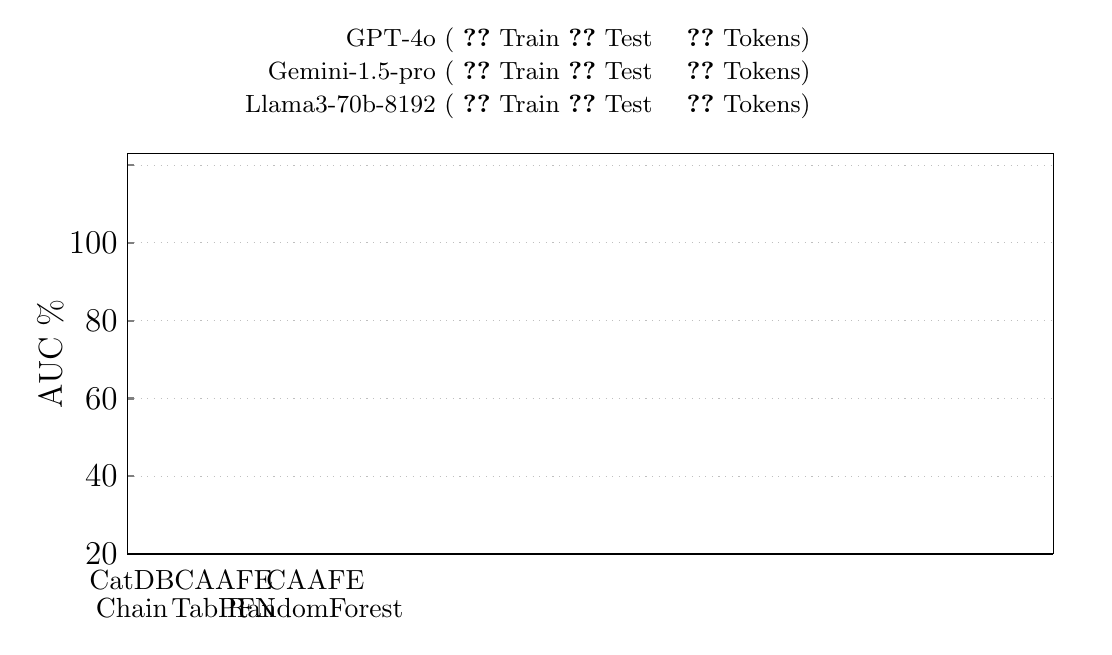
\begin{tikzpicture}[
  every axis/.style={
  height=0.55\columnwidth,
  width=1.1\columnwidth,  
  }]
 \begin{axis}[   
  axis y line*=left,	
  every major tick/.append style={ thick,major tick length=2.5pt, gray},
  axis line style={black},
  ybar,        
  ybar=0pt,
  ymin=0,
  ymax=1,
  log ticks with fixed point,
  y tick label style={/pgf/number format/1000 sep={}},
  x tick label style={/pgf/number format/1000 sep={}},
  scaled y ticks=false,
  enlarge y limits={0.03,upper},
  enlarge x limits=0.005,
  ylabel={AUC $\%$},
  xlabel={},
  ytick={0,0.2,0.4,0.6,0.8,1.0},
  yticklabels={0, 20, 40, 60, 80, 100},
  xtick style={draw=none},
  xtick pos=left,
  ytick pos=left,
  yticklabel style = {font=\large},
  ylabel style = {font=\large, yshift=-5pt},
  xticklabel style = {font=\normalsize, xshift=0pt, yshift=0pt, rotate=0},
  ymajorgrids,
  grid style=dotted,
  minor grid style={gray!80, dotted},
  nodes near coords,
  every node near coord/.style={font=\fontsize{0.1pt}{0.1}, rotate=0},
  every axis plot/.append style={line width=0.8pt,mark options={scale=1.5,solid}},  
  legend image post style={line width=.5pt},   
  boxplot/draw direction=y,
  boxplot={
      draw position={1 + floor(\plotnumofactualtype/24)+ 1/1*fpumod(\plotnumofactualtype,24)},
      box extend=0.85,
  },
  xtick={3,9,15,22},
  xticklabels={CatDB,\shortstack[c]{CatDB\\Chain},\shortstack[c]{CAAFE\\TabPFN},\shortstack[c]{CAAFE\\RandomForest}},
  legend image code/.code={\draw [#1] (0cm,-0.1cm) rectangle (0.2cm,0.1cm); },  
%}
]  
  \addboxplot{CatDB}{Tic-Tac-Toe}{gpt-4o}{}{dblue2}{dblue1};
  \addboxplot{CatDB}{Tic-Tac-Toe}{gemini-1.5-pro-latest}{}{dred2}{dred1};
  \addboxplot{CatDB}{Tic-Tac-Toe}{llama3-70b-8192}{}{teal2}{teal1};
  

  \addboxplot{CatDBChain}{Tic-Tac-Toe}{gpt-4o}{}{dblue2}{dblue1}
  \addboxplot{CatDBChain}{Tic-Tac-Toe}{gemini-1.5-pro-latest}{}{dred2}{dred1};
  \addboxplot{CatDBChain}{Tic-Tac-Toe}{llama3-70b-8192}{}{teal2}{teal1};
  

  \addboxplot{CAAFE}{Tic-Tac-Toe}{gpt-4o}{-TabPFN}{dblue2}{dblue1};
  \addboxplot{CAAFE}{Tic-Tac-Toe}{gemini-1.5-pro-latest}{-TabPFN}{dred2}{dred1};
  \addboxplot{CAAFE}{Balance-Scale}{llama3-70b-8192}{-TabPFN}{teal2}{teal1};
  
  \addboxplot{CAAFE}{Tic-Tac-Toe}{gpt-4o}{-RandomForest}{dblue2}{dblue1};
  \addboxplot{CAAFE}{Tic-Tac-Toe}{gemini-1.5-pro-latest}{-RandomForest}{dred2}{dred1};
  \addboxplot{CAAFE}{Tic-Tac-Toe}{llama3-70b-8192}{-RandomForest}{teal2}{teal1};
  
  \coordinate (top1) at (axis cs:6.49,\pgfkeysvalueof{/pgfplots/ymax});
  \coordinate (bot1) at (axis cs:6.49,\pgfkeysvalueof{/pgfplots/ymin});

  \coordinate (top2) at (axis cs:12.49,\pgfkeysvalueof{/pgfplots/ymax});
  \coordinate (bot2) at (axis cs:12.49,\pgfkeysvalueof{/pgfplots/ymin});

  \coordinate (top3) at (axis cs:18.49,\pgfkeysvalueof{/pgfplots/ymax});
  \coordinate (bot3) at (axis cs:18.49,\pgfkeysvalueof{/pgfplots/ymin});

  \draw[black!50, thick] (top1) -- (bot1);
  \draw[black!50, thick] (top2) -- (bot2);
  \draw[black!50, thick] (top3) -- (bot3);

  \draw[gray, densely dotted] (axis cs:2.5,\pgfkeysvalueof{/pgfplots/ymax}) -- (axis cs:2.5,\pgfkeysvalueof{/pgfplots/ymin});
  \draw[gray, densely dotted] (axis cs:4.45,\pgfkeysvalueof{/pgfplots/ymax}) -- (axis cs:4.45,\pgfkeysvalueof{/pgfplots/ymin});

  \draw[gray, densely dotted] (axis cs:8.55,\pgfkeysvalueof{/pgfplots/ymax}) -- (axis cs:8.55,\pgfkeysvalueof{/pgfplots/ymin});
  \draw[gray, densely dotted] (axis cs:10.5,\pgfkeysvalueof{/pgfplots/ymax}) -- (axis cs:10.5,\pgfkeysvalueof{/pgfplots/ymin});

  \draw[gray, densely dotted] (axis cs:14.6,\pgfkeysvalueof{/pgfplots/ymax}) -- (axis cs:14.6,\pgfkeysvalueof{/pgfplots/ymin});
  \draw[gray, densely dotted] (axis cs:16.55,\pgfkeysvalueof{/pgfplots/ymax}) -- (axis cs:16.55,\pgfkeysvalueof{/pgfplots/ymin});

  \draw[gray, densely dotted] (axis cs:20.65,\pgfkeysvalueof{/pgfplots/ymax}) -- (axis cs:20.65,\pgfkeysvalueof{/pgfplots/ymin});
  \draw[gray, densely dotted] (axis cs:22.6,\pgfkeysvalueof{/pgfplots/ymax}) -- (axis cs:22.6,\pgfkeysvalueof{/pgfplots/ymin});

\end{axis}

\begin{axis}[
  axis y line*=right,
  axis x line=none,  
  ybar,  
  ymin=0.5,
  y tick label style={/pgf/number format/1000 sep={}},
  x tick label style={/pgf/number format/1000 sep={}},
  scaled y ticks=false,
  enlarge y limits={1.3,upper},
  enlarge x limits=0.164,
  ylabel={},
  xlabel={},
  ytick={},
  yticklabels={},
  ytick style={draw=none},
  ytick align=outside,
  nodes near coords,
  nodes near coords align={vertical},
  every node near coord/.append style={font=\fontsize{7.5pt}{0.1}, rotate=90, xshift=-11pt, yshift=-6pt},%, rotate=90, xshift=-10pt, yshift=-5pt
  every axis plot/.append style={line width=0.8pt,mark options={scale=1.5,solid}},  
  legend image post style={line width=.5pt},   
  boxplot/draw direction=y,
  bar width=15pt,
  xtick = data,
  symbolic x coords={CatDB,CatDBChain, CAAFETabPFN,CAAFERandomForest},
  legend image code/.code={\draw [#1] (0cm,-0.1cm) rectangle (0.2cm,0.1cm); }, 
  ]   

    \addcost{Tic-Tac-Toe}{gpt-4o}{gray}{-.5pt};
    \addcost{Tic-Tac-Toe}{gemini-1.5-pro-latest}{lightgray}{0.5pt};
    \addcost{Tic-Tac-Toe}{llama3-70b-8192}{white}{1.4pt};
    
\end{axis}

\node [draw=none,inner sep=0, font=\small, anchor=west] (leg1) at (rel axis cs: 0.25,1.20) {\shortstack[r]{
  GPT-4o ( \ref{gpt-4o_CatDB_train} Train \ref{gpt-4o_CatDB_test} Test \ \ \ \ref{gpt-4o} Tokens) \\
  Gemini-1.5-pro ( \ref{gemini-1.5-pro-latest_CatDB_train} Train \ref{gemini-1.5-pro-latest_CatDB_test} Test \ \ \ \ref{gemini-1.5-pro-latest} Tokens) \\
  Llama3-70b-8192 ( \ref{llama3-70b-8192_CatDB_train} Train \ref{llama3-70b-8192_CatDB_test} Test \ \ \ \ref{llama3-70b-8192} Tokens)  
  }};

\end{tikzpicture}
            \caption{Experiment1-Performance-Tic-Tac-Toe}
        \end{figure}  
    
  
    \tikzsetnextfilename{Experiment1-Performance-Eucalyptus} 
        \begin{figure}[!ht]
            \centering
            \pgfmathdeclarefunction{fpumod}{2}{%
        \pgfmathfloatdivide{#1}{#2}%
        \pgfmathfloatint{\pgfmathresult}%
        \pgfmathfloatmultiply{\pgfmathresult}{#2}%
        \pgfmathfloatsubtract{#1}{\pgfmathresult}%
        % replaced `0' by `5' to make it work for this problem
        \pgfmathfloatifapproxequalrel{\pgfmathresult}{#2}{\def\pgfmathresult{5}}{}%
}

\newcommand{\myaddplot}[6]{
  \addplot[xshift=0pt,boxplot,fill=#4, draw=#4, mark options={scale=0.5, fill=#4}, line width=1.5pt] 
  table[y=#2, col sep=comma, x=ID]{#3};
  \label{#5_#6_#1}    
};
    
\newcommand{\addboxplot}[6]{
  \myaddplot{train}{train_auc_ovr}{../archive/SIGMOD2025-Results/seperate/#1-#2-#3#4-No.csv}{#5}{#3}{#1};
  \myaddplot{test}{test_auc_ovr}{../archive/SIGMOD2025-Results/seperate/#1-#2-#3#4-No.csv}{#6}{#3}{#1};
};

\newcommand{\myaddplotcost}[4]{ %postaction={pattern=horizontal lines, pattern color=#3}
  \addplot[xshift=#4,fill=#3, draw=black,line width=0.3pt] table[x=config, col sep=comma, y=tokens_count, discard if singlconfig={#1}{#2}]{../archive/SIGMOD2025-Results/CostResults.csv};
  \label{#2}    
};

\newcommand{\addcost}[4]{
  \myaddplotcost{#1}{#2}{#3}{#4};
};


\pgfplotsset{
    discard if singlconfig/.style n args={2}{
        x filter/.code={
            \edef\tempa{\thisrow{dataset_name_orig}}
            \edef\tempb{#1}
            \ifx\tempa\tempb
              \edef\tempc{\thisrow{llm_model}}
                \edef\tempd{#2}
                  \ifx\tempc\tempd                  
                  \else
                  \def\pgfmathresult{inf}
                  \fi
            \else
            \def\pgfmathresult{inf}
            \fi			
        }
    },
};

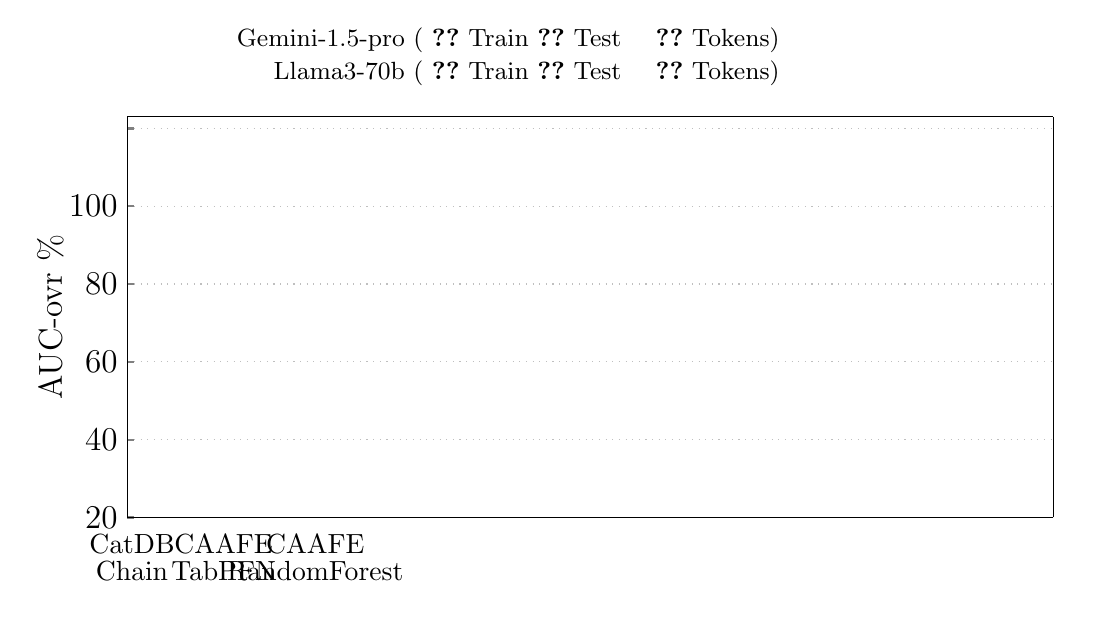
\begin{tikzpicture}[
  every axis/.style={
  height=0.55\columnwidth,
  width=1.1\columnwidth,  
  }]
 \begin{axis}[   
  axis y line*=left,	
  every major tick/.append style={ thick,major tick length=2.5pt, gray},
  axis line style={black},
  ybar,        
  ybar=0pt,
  ymin=0,
  ymax=1,
  log ticks with fixed point,
  y tick label style={/pgf/number format/1000 sep={}},
  x tick label style={/pgf/number format/1000 sep={}},
  scaled y ticks=false,
  enlarge y limits={0.03,upper},
  enlarge x limits=0.005,
  ylabel={AUC-ovr $\%$},
  xlabel={},
  ytick={0,0.2,0.4,0.6,0.8,1.0},
  yticklabels={0, 20, 40, 60, 80, 100},
  xtick style={draw=none},
  xtick pos=left,
  ytick pos=left,
  yticklabel style = {font=\large},
  ylabel style = {font=\large, yshift=-5pt},
  xticklabel style = {font=\normalsize, xshift=0pt, yshift=0pt, rotate=0},
  ymajorgrids,
  grid style=dotted,
  minor grid style={gray!80, dotted},
  nodes near coords,
  every node near coord/.style={font=\fontsize{0.1pt}{0.1}, rotate=0},
  every axis plot/.append style={line width=0.8pt,mark options={scale=1.5,solid}},  
  legend image post style={line width=.5pt},   
  boxplot/draw direction=y,
  boxplot={
      draw position={1 + floor(\plotnumofactualtype/24)+ 1/1*fpumod(\plotnumofactualtype,24)},
      box extend=0.85,
  },
  xtick={3,9,15,22},
  xticklabels={CatDB,\shortstack[c]{CatDB\\Chain},\shortstack[c]{CAAFE\\TabPFN},\shortstack[c]{CAAFE\\RandomForest}},
  legend image code/.code={\draw [#1] (0cm,-0.1cm) rectangle (0.2cm,0.1cm); },  
%}
]  
  \addboxplot{CatDB}{Eucalyptus-rnc}{gemini-1.5-pro-latest}{}{white}{white}; %{color4!60}{color4}
  \addboxplot{CatDB}{Eucalyptus-rnc}{gemini-1.5-pro-latest}{}{tug!50}{tug};
  \addboxplot{CatDB}{Eucalyptus-rnc}{llama3-70b-8192}{}{tugb}{tugb!150};
  

  \addboxplot{CatDBChain}{Eucalyptus-rnc}{gemini-1.5-pro-latest}{}{white}{white};
  \addboxplot{CatDBChain}{Eucalyptus-rnc}{gemini-1.5-pro-latest}{}{tug!50}{tug};
  \addboxplot{CatDBChain}{Eucalyptus-rnc}{llama3-70b-8192}{}{tugb}{tugb!150};
  

  \addboxplot{CAAFE}{Eucalyptus-rnc}{gemini-1.5-pro-latest}{-TabPFN}{white}{white};
  \addboxplot{CAAFE}{Eucalyptus-rnc}{gemini-1.5-pro-latest}{-TabPFN}{tug!50}{tug};
  \addboxplot{CAAFE}{Eucalyptus-rnc}{gemini-1.5-pro-latest}{-TabPFN}{white}{white};
  
  \addboxplot{CAAFE}{Eucalyptus-rnc}{gemini-1.5-pro-latest}{-RandomForest}{white}{white};
  \addboxplot{CAAFE}{Eucalyptus-rnc}{gemini-1.5-pro-latest}{-RandomForest}{tug!50}{tug};
  \addboxplot{CAAFE}{Eucalyptus-rnc}{gemini-1.5-pro-latest}{-RandomForest}{white}{white};
  

  \draw[black!50, thick] (59,0) -- (59,103);
  \draw[black!50, thick] (119,0) -- (119,103);
  \draw[black!50, thick] (179,0) -- (179,103);

\end{axis}

\begin{axis}[
  axis y line*=right,
  axis x line=none,  
  ybar,  
  ymin=0.5,
  y tick label style={/pgf/number format/1000 sep={}},
  x tick label style={/pgf/number format/1000 sep={}},
  scaled y ticks=false,
  enlarge y limits={1.3,upper},
  enlarge x limits=0.18,
  ylabel={},
  xlabel={},
  ytick={},
  yticklabels={},
  ytick style={draw=none},
  ytick align=outside,
  nodes near coords,
  nodes near coords align={vertical},
  every node near coord/.append style={font=\fontsize{7.5pt}{0.1}, rotate=90, xshift=-11pt, yshift=-6pt},%, rotate=90, xshift=-10pt, yshift=-5pt
  every axis plot/.append style={line width=0.8pt,mark options={scale=1.5,solid}},  
  legend image post style={line width=.5pt},   
  boxplot/draw direction=y,
  bar width=13pt,
  xtick = data,
  symbolic x coords={CatDB,CatDBChain, CAAFETabPFN,CAAFERandomForest},
  legend image code/.code={\draw [#1] (0cm,-0.1cm) rectangle (0.2cm,0.1cm); }, 
  ]   

    %\addcost{Eucalyptus-rnc}{gemini-1.5-pro-latest}{lightgray!120}{0pt};
    \addcost{Eucalyptus-rnc}{gemini-1.5-pro-latest}{white}{0pt};
    \addcost{Eucalyptus-rnc}{llama3-70b-8192}{lightgray!70}{0pt};
    
\end{axis}

\node [draw=none,inner sep=0, font=\small, anchor=west] (leg1) at (rel axis cs: 0.25,1.15) {\shortstack[r]{
  Gemini-1.5-pro ( \ref{gemini-1.5-pro-latest_CatDB_train} Train \ref{gemini-1.5-pro-latest_CatDB_test} Test \ \ \ \ref{gemini-1.5-pro-latest} Tokens) \\
  Llama3-70b ( \ref{llama3-70b-8192_CatDB_train} Train \ref{llama3-70b-8192_CatDB_test} Test \ \ \ \ref{llama3-70b-8192} Tokens)}};

\end{tikzpicture}
            \caption{Experiment1-Performance-Eucalyptus}
        \end{figure}  
    
  
    \tikzsetnextfilename{Experiment1-Performance-PC1} 
        \begin{figure}[!ht]
            \centering
            \pgfmathdeclarefunction{fpumod}{2}{%
        \pgfmathfloatdivide{#1}{#2}%
        \pgfmathfloatint{\pgfmathresult}%
        \pgfmathfloatmultiply{\pgfmathresult}{#2}%
        \pgfmathfloatsubtract{#1}{\pgfmathresult}%
        % replaced `0' by `5' to make it work for this problem
        \pgfmathfloatifapproxequalrel{\pgfmathresult}{#2}{\def\pgfmathresult{5}}{}%
}

\newcommand{\myaddplot}[6]{
  \addplot[xshift=0pt,boxplot,fill=#4, draw=#4, mark options={scale=0.5, fill=#4}, line width=1.5pt] 
  table[y=#2, col sep=comma, x=ID]{#3};
  \label{#5_#6_#1}    
};
    
\newcommand{\addboxplot}[6]{
  \myaddplot{train}{train_auc}{../archive/SIGMOD2025-Results/seperate/#1-#2-#3#4-No.csv}{#5}{#3}{#1};
  \myaddplot{test}{test_auc}{../archive/SIGMOD2025-Results/seperate/#1-#2-#3#4-No.csv}{#6}{#3}{#1};
};

\newcommand{\myaddplotcost}[4]{ %postaction={pattern=horizontal lines, pattern color=#3}
  \addplot[xshift=#4,fill=#3, draw=black,line width=0.3pt] table[x=config, col sep=comma, y=tokens_count, discard if singlconfig={#1}{#2}]{../archive/SIGMOD2025-Results/CostResults.csv};
  \label{#2}    
};

\newcommand{\addcost}[4]{
  \myaddplotcost{#1}{#2}{#3}{#4};
};


\pgfplotsset{
    discard if singlconfig/.style n args={2}{
        x filter/.code={
            \edef\tempa{\thisrow{dataset_name_orig}}
            \edef\tempb{#1}
            \ifx\tempa\tempb
              \edef\tempc{\thisrow{llm_model}}
                \edef\tempd{#2}
                  \ifx\tempc\tempd                  
                  \else
                  \def\pgfmathresult{inf}
                  \fi
            \else
            \def\pgfmathresult{inf}
            \fi			
        }
    },
};

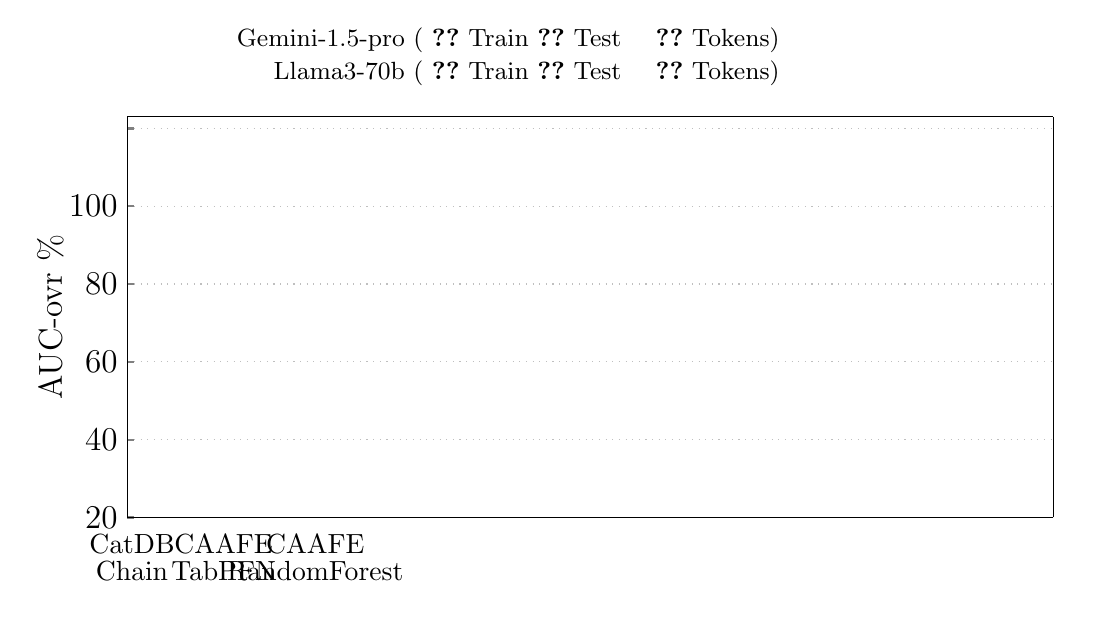
\begin{tikzpicture}[
  every axis/.style={
  height=0.55\columnwidth,
  width=1.1\columnwidth,  
  }]
 \begin{axis}[   
  axis y line*=left,	
  every major tick/.append style={ thick,major tick length=2.5pt, gray},
  axis line style={black},
  ybar,        
  ybar=0pt,
  ymin=0,
  ymax=1,
  log ticks with fixed point,
  y tick label style={/pgf/number format/1000 sep={}},
  x tick label style={/pgf/number format/1000 sep={}},
  scaled y ticks=false,
  enlarge y limits={0.03,upper},
  enlarge x limits=0.005,
  ylabel={AUC-ovr $\%$},
  xlabel={},
  ytick={0,0.2,0.4,0.6,0.8,1.0},
  yticklabels={0, 20, 40, 60, 80, 100},
  xtick style={draw=none},
  xtick pos=left,
  ytick pos=left,
  yticklabel style = {font=\large},
  ylabel style = {font=\large, yshift=-5pt},
  xticklabel style = {font=\normalsize, xshift=0pt, yshift=0pt, rotate=0},
  ymajorgrids,
  grid style=dotted,
  minor grid style={gray!80, dotted},
  nodes near coords,
  every node near coord/.style={font=\fontsize{0.1pt}{0.1}, rotate=0},
  every axis plot/.append style={line width=0.8pt,mark options={scale=1.5,solid}},  
  legend image post style={line width=.5pt},   
  boxplot/draw direction=y,
  boxplot={
      draw position={1 + floor(\plotnumofactualtype/24)+ 1/1*fpumod(\plotnumofactualtype,24)},
      box extend=0.85,
  },
  xtick={3,9,15,22},
  xticklabels={CatDB,\shortstack[c]{CatDB\\Chain},\shortstack[c]{CAAFE\\TabPFN},\shortstack[c]{CAAFE\\RandomForest}},
  legend image code/.code={\draw [#1] (0cm,-0.1cm) rectangle (0.2cm,0.1cm); },  
%}
]  
  \addboxplot{CatDB}{PC1-rnc}{gemini-1.5-pro-latest}{}{white}{white}; %{color4!60}{color4}
  \addboxplot{CatDB}{PC1-rnc}{gemini-1.5-pro-latest}{}{tug!50}{tug};
  \addboxplot{CatDB}{PC1-rnc}{llama3-70b-8192}{}{tugb}{tugb!150};
  

  \addboxplot{CatDBChain}{PC1-rnc}{gemini-1.5-pro-latest}{}{white}{white};
  \addboxplot{CatDBChain}{PC1-rnc}{gemini-1.5-pro-latest}{}{tug!50}{tug};
  \addboxplot{CatDBChain}{PC1-rnc}{llama3-70b-8192}{}{tugb}{tugb!150};
  

  \addboxplot{CAAFE}{PC1-rnc}{gemini-1.5-pro-latest}{-TabPFN}{white}{white};
  \addboxplot{CAAFE}{PC1-rnc}{gemini-1.5-pro-latest}{-TabPFN}{tug!50}{tug};
  \addboxplot{CAAFE}{PC1-rnc}{gemini-1.5-pro-latest}{-TabPFN}{white}{white};
  
  \addboxplot{CAAFE}{PC1-rnc}{gemini-1.5-pro-latest}{-RandomForest}{white}{white};
  \addboxplot{CAAFE}{PC1-rnc}{gemini-1.5-pro-latest}{-RandomForest}{tug!50}{tug};
  \addboxplot{CAAFE}{PC1-rnc}{gemini-1.5-pro-latest}{-RandomForest}{white}{white};
  

  \draw[black!50, thick] (59,0) -- (59,103);
  \draw[black!50, thick] (119,0) -- (119,103);
  \draw[black!50, thick] (179,0) -- (179,103);

\end{axis}

\begin{axis}[
  axis y line*=right,
  axis x line=none,  
  ybar,  
  ymin=0.5,
  y tick label style={/pgf/number format/1000 sep={}},
  x tick label style={/pgf/number format/1000 sep={}},
  scaled y ticks=false,
  enlarge y limits={1.3,upper},
  enlarge x limits=0.18,
  ylabel={},
  xlabel={},
  ytick={},
  yticklabels={},
  ytick style={draw=none},
  ytick align=outside,
  nodes near coords,
  nodes near coords align={vertical},
  every node near coord/.append style={font=\fontsize{7.5pt}{0.1}, rotate=90, xshift=-11pt, yshift=-6pt},%, rotate=90, xshift=-10pt, yshift=-5pt
  every axis plot/.append style={line width=0.8pt,mark options={scale=1.5,solid}},  
  legend image post style={line width=.5pt},   
  boxplot/draw direction=y,
  bar width=13pt,
  xtick = data,
  symbolic x coords={CatDB,CatDBChain, CAAFETabPFN,CAAFERandomForest},
  legend image code/.code={\draw [#1] (0cm,-0.1cm) rectangle (0.2cm,0.1cm); }, 
  ]   

    %\addcost{PC1-rnc}{gemini-1.5-pro-latest}{lightgray!120}{0pt};
    \addcost{PC1-rnc}{gemini-1.5-pro-latest}{white}{0pt};
    \addcost{PC1-rnc}{llama3-70b-8192}{lightgray!70}{0pt};
    
\end{axis}

\node [draw=none,inner sep=0, font=\small, anchor=west] (leg1) at (rel axis cs: 0.25,1.15) {\shortstack[r]{
  Gemini-1.5-pro ( \ref{gemini-1.5-pro-latest_CatDB_train} Train \ref{gemini-1.5-pro-latest_CatDB_test} Test \ \ \ \ref{gemini-1.5-pro-latest} Tokens) \\
  Llama3-70b ( \ref{llama3-70b-8192_CatDB_train} Train \ref{llama3-70b-8192_CatDB_test} Test \ \ \ \ref{llama3-70b-8192} Tokens)}};

\end{tikzpicture}
            \caption{Experiment1-Performance-PC1}
        \end{figure}  
    
  
    % \tikzsetnextfilename{Experiment1-Performance-Airlines} 
    %     \begin{figure}[!ht]
    %         \centering
    %         \pgfmathdeclarefunction{fpumod}{2}{%
        \pgfmathfloatdivide{#1}{#2}%
        \pgfmathfloatint{\pgfmathresult}%
        \pgfmathfloatmultiply{\pgfmathresult}{#2}%
        \pgfmathfloatsubtract{#1}{\pgfmathresult}%
        % replaced `0' by `5' to make it work for this problem
        \pgfmathfloatifapproxequalrel{\pgfmathresult}{#2}{\def\pgfmathresult{5}}{}%
}

\newcommand{\myaddplot}[6]{
  \addplot[xshift=0pt,boxplot,fill=#4, draw=#4, mark options={scale=0.5, fill=#4}, line width=1.5pt] 
  table[y=#2, col sep=comma, x=ID]{#3};
  \label{#5_#6_#1}    
};
    
\newcommand{\addboxplot}[6]{
  \myaddplot{train}{train_auc}{../archive/SIGMOD2025-Results/seperate/#1-#2-#3#4-No.csv}{#5}{#3}{#1};
  \myaddplot{test}{test_auc}{../archive/SIGMOD2025-Results/seperate/#1-#2-#3#4-No.csv}{#6}{#3}{#1};
};

\newcommand{\myaddplotcost}[4]{ %postaction={pattern=horizontal lines, pattern color=#3}
  \addplot[xshift=#4,fill=#3, draw=black,line width=0.3pt] table[x=config, col sep=comma, y=tokens_count, discard if singlconfig={#1}{#2}]{../archive/SIGMOD2025-Results/CostResults.csv};
  \label{#2}    
};

\newcommand{\addcost}[4]{
  \myaddplotcost{#1}{#2}{#3}{#4};
};


\pgfplotsset{
    discard if singlconfig/.style n args={2}{
        x filter/.code={
            \edef\tempa{\thisrow{dataset_name_orig}}
            \edef\tempb{#1}
            \ifx\tempa\tempb
              \edef\tempc{\thisrow{llm_model}}
                \edef\tempd{#2}
                  \ifx\tempc\tempd                  
                  \else
                  \def\pgfmathresult{inf}
                  \fi
            \else
            \def\pgfmathresult{inf}
            \fi			
        }
    },
};

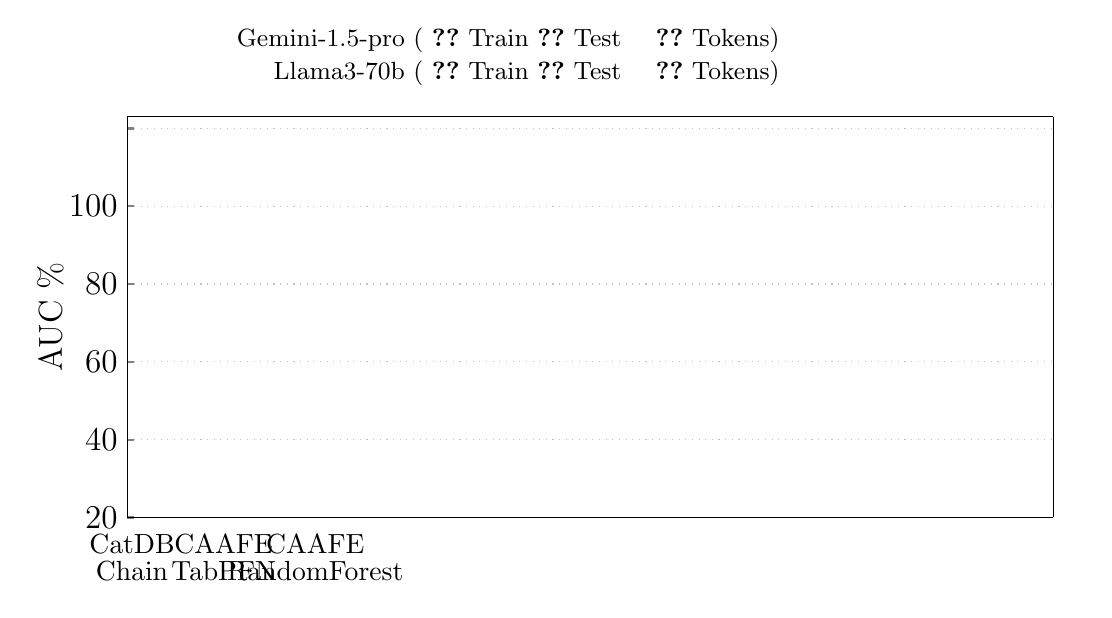
\begin{tikzpicture}[
  every axis/.style={
  height=0.55\columnwidth,
  width=1.1\columnwidth,  
  }]
 \begin{axis}[   
  axis y line*=left,	
  every major tick/.append style={ thick,major tick length=2.5pt, gray},
  axis line style={black},
  ybar,        
  ybar=0pt,
  ymin=0,
  ymax=1,
  log ticks with fixed point,
  y tick label style={/pgf/number format/1000 sep={}},
  x tick label style={/pgf/number format/1000 sep={}},
  scaled y ticks=false,
  enlarge y limits={0.03,upper},
  enlarge x limits=0.005,
  ylabel={AUC $\%$},
  xlabel={},
  ytick={0,0.2,0.4,0.6,0.8,1.0},
  yticklabels={0, 20, 40, 60, 80, 100},
  xtick style={draw=none},
  xtick pos=left,
  ytick pos=left,
  yticklabel style = {font=\large},
  ylabel style = {font=\large, yshift=-5pt},
  xticklabel style = {font=\normalsize, xshift=0pt, yshift=0pt, rotate=0},
  ymajorgrids,
  grid style=dotted,
  minor grid style={gray!80, dotted},
  nodes near coords,
  every node near coord/.style={font=\fontsize{0.1pt}{0.1}, rotate=0},
  every axis plot/.append style={line width=0.8pt,mark options={scale=1.5,solid}},  
  legend image post style={line width=.5pt},   
  boxplot/draw direction=y,
  boxplot={
      draw position={1 + floor(\plotnumofactualtype/24)+ 1/1*fpumod(\plotnumofactualtype,24)},
      box extend=0.85,
  },
  xtick={3,9,15,22},
  xticklabels={CatDB,\shortstack[c]{CatDB\\Chain},\shortstack[c]{CAAFE\\TabPFN},\shortstack[c]{CAAFE\\RandomForest}},
  legend image code/.code={\draw [#1] (0cm,-0.1cm) rectangle (0.2cm,0.1cm); },  
%}
]  
  \addboxplot{CatDB}{Airlines-rnc}{gemini-1.5-pro-latest}{}{white}{white}; %{color4!60}{color4}
  \addboxplot{CatDB}{Airlines-rnc}{gemini-1.5-pro-latest}{}{tug!50}{tug};
  \addboxplot{CatDB}{Airlines-rnc}{llama3-70b-8192}{}{tugb}{tugb!150};
  

  \addboxplot{CatDBChain}{Airlines-rnc}{gemini-1.5-pro-latest}{}{white}{white};
  \addboxplot{CatDBChain}{Airlines-rnc}{gemini-1.5-pro-latest}{}{tug!50}{tug};
  \addboxplot{CatDBChain}{Airlines-rnc}{llama3-70b-8192}{}{tugb}{tugb!150};
  

  \addboxplot{CAAFE}{Airlines-rnc}{gemini-1.5-pro-latest}{-TabPFN}{white}{white};
  \addboxplot{CAAFE}{Airlines-rnc}{gemini-1.5-pro-latest}{-TabPFN}{tug!50}{tug};
  \addboxplot{CAAFE}{Airlines-rnc}{gemini-1.5-pro-latest}{-TabPFN}{white}{white};
  
  \addboxplot{CAAFE}{Airlines-rnc}{gemini-1.5-pro-latest}{-RandomForest}{white}{white};
  \addboxplot{CAAFE}{Airlines-rnc}{gemini-1.5-pro-latest}{-RandomForest}{tug!50}{tug};
  \addboxplot{CAAFE}{Airlines-rnc}{gemini-1.5-pro-latest}{-RandomForest}{white}{white};
  

  \draw[black!50, thick] (59,0) -- (59,103);
  \draw[black!50, thick] (119,0) -- (119,103);
  \draw[black!50, thick] (179,0) -- (179,103);

\end{axis}

\begin{axis}[
  axis y line*=right,
  axis x line=none,  
  ybar,  
  ymin=0.5,
  y tick label style={/pgf/number format/1000 sep={}},
  x tick label style={/pgf/number format/1000 sep={}},
  scaled y ticks=false,
  enlarge y limits={1.3,upper},
  enlarge x limits=0.18,
  ylabel={},
  xlabel={},
  ytick={},
  yticklabels={},
  ytick style={draw=none},
  ytick align=outside,
  nodes near coords,
  nodes near coords align={vertical},
  every node near coord/.append style={font=\fontsize{7.5pt}{0.1}, rotate=90, xshift=-11pt, yshift=-6pt},%, rotate=90, xshift=-10pt, yshift=-5pt
  every axis plot/.append style={line width=0.8pt,mark options={scale=1.5,solid}},  
  legend image post style={line width=.5pt},   
  boxplot/draw direction=y,
  bar width=13pt,
  xtick = data,
  symbolic x coords={CatDB,CatDBChain, CAAFETabPFN,CAAFERandomForest},
  legend image code/.code={\draw [#1] (0cm,-0.1cm) rectangle (0.2cm,0.1cm); }, 
  ]   

    %\addcost{Airlines-rnc}{gemini-1.5-pro-latest}{color8!10}{0pt};
    \addcost{Airlines-rnc}{gemini-1.5-pro-latest}{color8!40}{0pt};
    \addcost{Airlines-rnc}{llama3-70b-8192}{color8!70!}{0pt};
    
\end{axis}

\node [draw=none,inner sep=0, font=\small, anchor=west] (leg1) at (rel axis cs: 0.25,1.15) {\shortstack[r]{
  Gemini-1.5-pro ( \ref{gemini-1.5-pro-latest_CatDB_train} Train \ref{gemini-1.5-pro-latest_CatDB_test} Test \ \ \ \ref{gemini-1.5-pro-latest} Tokens) \\
  Llama3-70b ( \ref{llama3-70b-8192_CatDB_train} Train \ref{llama3-70b-8192_CatDB_test} Test \ \ \ \ref{llama3-70b-8192} Tokens)}};

\end{tikzpicture}
    %         \caption{Experiment1-Performance-Airlines}
    %     \end{figure}  
    
  
    \tikzsetnextfilename{Experiment1-Performance-Jungle-Chess} 
        \begin{figure}[!ht]
            \centering
            \pgfmathdeclarefunction{fpumod}{2}{%
        \pgfmathfloatdivide{#1}{#2}%
        \pgfmathfloatint{\pgfmathresult}%
        \pgfmathfloatmultiply{\pgfmathresult}{#2}%
        \pgfmathfloatsubtract{#1}{\pgfmathresult}%
        % replaced `0' by `5' to make it work for this problem
        \pgfmathfloatifapproxequalrel{\pgfmathresult}{#2}{\def\pgfmathresult{5}}{}%
}

\newcommand{\myaddplot}[6]{
  \addplot[xshift=0pt,boxplot,fill=#4, draw=#4, mark options={scale=0.5, fill=#4}, line width=1.5pt] 
  table[y=#2, col sep=comma, x=ID]{#3};
  \label{#5_#6_#1}    
};
    
\newcommand{\addboxplot}[6]{
  \myaddplot{train}{train_auc_ovr}{../archive/SIGMOD2025-Results/seperate/#1-#2-#3#4-No.csv}{#5}{#3}{#1};
  \myaddplot{test}{test_auc_ovr}{../archive/SIGMOD2025-Results/seperate/#1-#2-#3#4-No.csv}{#6}{#3}{#1};
};

\newcommand{\myaddplotcost}[4]{ %postaction={pattern=horizontal lines, pattern color=#3}
  \addplot[xshift=#4,fill=#3, draw=black,line width=0.3pt] table[x=config, col sep=comma, y=tokens_count, discard if singlconfig={#1}{#2}]{../archive/SIGMOD2025-Results/CostResults.csv};
  \label{#2}    
};

\newcommand{\addcost}[4]{
  \myaddplotcost{#1}{#2}{#3}{#4};
};


\pgfplotsset{
    discard if singlconfig/.style n args={2}{
        x filter/.code={
            \edef\tempa{\thisrow{dataset_name_orig}}
            \edef\tempb{#1}
            \ifx\tempa\tempb
              \edef\tempc{\thisrow{llm_model}}
                \edef\tempd{#2}
                  \ifx\tempc\tempd                  
                  \else
                  \def\pgfmathresult{inf}
                  \fi
            \else
            \def\pgfmathresult{inf}
            \fi			
        }
    },
};

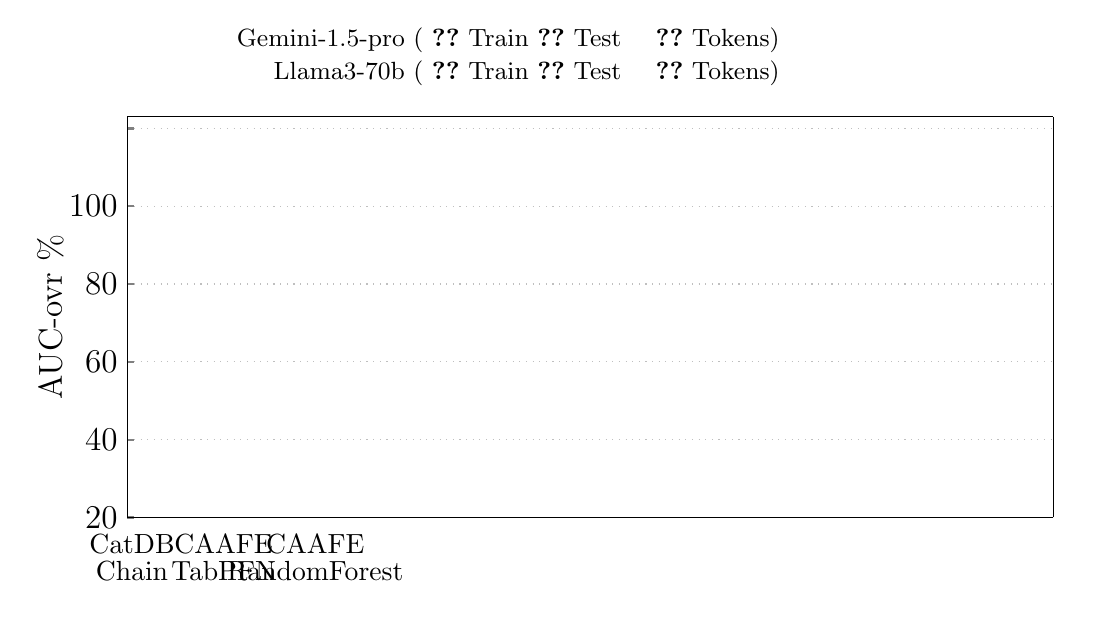
\begin{tikzpicture}[
  every axis/.style={
  height=0.55\columnwidth,
  width=1.1\columnwidth,  
  }]
 \begin{axis}[   
  axis y line*=left,	
  every major tick/.append style={ thick,major tick length=2.5pt, gray},
  axis line style={black},
  ybar,        
  ybar=0pt,
  ymin=0,
  ymax=1,
  log ticks with fixed point,
  y tick label style={/pgf/number format/1000 sep={}},
  x tick label style={/pgf/number format/1000 sep={}},
  scaled y ticks=false,
  enlarge y limits={0.03,upper},
  enlarge x limits=0.005,
  ylabel={AUC-ovr $\%$},
  xlabel={},
  ytick={0,0.2,0.4,0.6,0.8,1.0},
  yticklabels={0, 20, 40, 60, 80, 100},
  xtick style={draw=none},
  xtick pos=left,
  ytick pos=left,
  yticklabel style = {font=\large},
  ylabel style = {font=\large, yshift=-5pt},
  xticklabel style = {font=\normalsize, xshift=0pt, yshift=0pt, rotate=0},
  ymajorgrids,
  grid style=dotted,
  minor grid style={gray!80, dotted},
  nodes near coords,
  every node near coord/.style={font=\fontsize{0.1pt}{0.1}, rotate=0},
  every axis plot/.append style={line width=0.8pt,mark options={scale=1.5,solid}},  
  legend image post style={line width=.5pt},   
  boxplot/draw direction=y,
  boxplot={
      draw position={1 + floor(\plotnumofactualtype/24)+ 1/1*fpumod(\plotnumofactualtype,24)},
      box extend=0.85,
  },
  xtick={3,9,15,22},
  xticklabels={CatDB,\shortstack[c]{CatDB\\Chain},\shortstack[c]{CAAFE\\TabPFN},\shortstack[c]{CAAFE\\RandomForest}},
  legend image code/.code={\draw [#1] (0cm,-0.1cm) rectangle (0.2cm,0.1cm); },  
%}
]  
  \addboxplot{CatDB}{Jungle-Chess-rnc}{gemini-1.5-pro-latest}{}{white}{white}; %{color4!60}{color4}
  \addboxplot{CatDB}{Jungle-Chess-rnc}{gemini-1.5-pro-latest}{}{tug!50}{tug};
  \addboxplot{CatDB}{Jungle-Chess-rnc}{llama3-70b-8192}{}{tugb}{tugb!150};
  

  \addboxplot{CatDBChain}{Jungle-Chess-rnc}{gemini-1.5-pro-latest}{}{white}{white};
  \addboxplot{CatDBChain}{Jungle-Chess-rnc}{gemini-1.5-pro-latest}{}{tug!50}{tug};
  \addboxplot{CatDBChain}{Jungle-Chess-rnc}{llama3-70b-8192}{}{tugb}{tugb!150};
  

  \addboxplot{CAAFE}{Jungle-Chess-rnc}{gemini-1.5-pro-latest}{-TabPFN}{white}{white};
  \addboxplot{CAAFE}{Jungle-Chess-rnc}{gemini-1.5-pro-latest}{-TabPFN}{tug!50}{tug};
  \addboxplot{CAAFE}{Jungle-Chess-rnc}{gemini-1.5-pro-latest}{-TabPFN}{white}{white};
  
  \addboxplot{CAAFE}{Jungle-Chess-rnc}{gemini-1.5-pro-latest}{-RandomForest}{white}{white};
  \addboxplot{CAAFE}{Jungle-Chess-rnc}{gemini-1.5-pro-latest}{-RandomForest}{tug!50}{tug};
  \addboxplot{CAAFE}{Jungle-Chess-rnc}{gemini-1.5-pro-latest}{-RandomForest}{white}{white};
  

  \draw[black!50, thick] (59,0) -- (59,103);
  \draw[black!50, thick] (119,0) -- (119,103);
  \draw[black!50, thick] (179,0) -- (179,103);

\end{axis}

\begin{axis}[
  axis y line*=right,
  axis x line=none,  
  ybar,  
  ymin=0.5,
  y tick label style={/pgf/number format/1000 sep={}},
  x tick label style={/pgf/number format/1000 sep={}},
  scaled y ticks=false,
  enlarge y limits={1.3,upper},
  enlarge x limits=0.18,
  ylabel={},
  xlabel={},
  ytick={},
  yticklabels={},
  ytick style={draw=none},
  ytick align=outside,
  nodes near coords,
  nodes near coords align={vertical},
  every node near coord/.append style={font=\fontsize{7.5pt}{0.1}, rotate=90, xshift=-11pt, yshift=-6pt},%, rotate=90, xshift=-10pt, yshift=-5pt
  every axis plot/.append style={line width=0.8pt,mark options={scale=1.5,solid}},  
  legend image post style={line width=.5pt},   
  boxplot/draw direction=y,
  bar width=13pt,
  xtick = data,
  symbolic x coords={CatDB,CatDBChain, CAAFETabPFN,CAAFERandomForest},
  legend image code/.code={\draw [#1] (0cm,-0.1cm) rectangle (0.2cm,0.1cm); }, 
  ]   

    %\addcost{Jungle-Chess-rnc}{gemini-1.5-pro-latest}{color8!10}{0pt};
    \addcost{Jungle-Chess-rnc}{gemini-1.5-pro-latest}{color8!40}{0pt};
    \addcost{Jungle-Chess-rnc}{llama3-70b-8192}{color8!70!}{0pt};
    
\end{axis}

\node [draw=none,inner sep=0, font=\small, anchor=west] (leg1) at (rel axis cs: 0.25,1.15) {\shortstack[r]{
  Gemini-1.5-pro ( \ref{gemini-1.5-pro-latest_CatDB_train} Train \ref{gemini-1.5-pro-latest_CatDB_test} Test \ \ \ \ref{gemini-1.5-pro-latest} Tokens) \\
  Llama3-70b ( \ref{llama3-70b-8192_CatDB_train} Train \ref{llama3-70b-8192_CatDB_test} Test \ \ \ \ref{llama3-70b-8192} Tokens)}};

\end{tikzpicture}
            \caption{Experiment1-Performance-Jungle-Chess}
        \end{figure}  
    

\end{document}
\endinput
